\documentclass[a5paper, oneside]{book}
\usepackage[T2A]{fontenc}
\usepackage[utf8]{inputenc}   %кодировка
\usepackage[russian]{babel}   %язык
\usepackage{wrapfig}  %обтекание
\usepackage{graphicx}   %графика
\graphicspath{{OldPictures/}}   %папка с картинками 
\usepackage{amsmath}
\usepackage{amssymb}
\usepackage{indentfirst} %отступ в первом абзаце
\usepackage{subcaption}   %несколько фрагментов на рисунке
\usepackage[left=1.5cm,right=1.5cm,bottom=2cm]{geometry} %настройка полей
\usepackage{answers} %условия, решения и ответы печатаются в разных частях документа
\headsep=3mm   %расстояние между верхним колонтитулом и текстом
\Newassociation{sol}{Solution}{solutions}
\Newassociation{ans}{Answer}{answers}
\renewcommand{\Solutionlabel}[1]{\bf{Решение #1}}
\newtheorem{Exc}{Задача}
\newenvironment{ex}{\begin{Exc}\normalfont}{\end{Exc}}
\title{Сборник задач для подготовки к физическим олимпиадам}
\date{\today}

\begin{document}
\maketitle
\tableofcontents

\chapter*{Предисловие}\addcontentsline{toc}{chapter}{Предисловие} 
������������ ������� �������� � ���� ���������� ������, ������� � ������ ���� ������������ ���������, ������������� � ������ ������������ �� ������� ����� ���������� ��������� �� ���������� ���������� ��������� ���������������� ������������� ������������������ ������������. � ������� �������� ������� ������������ ����������� �� ������, ������������� � �������� ������������ � 2006 ����. ������ ����� �������� ��������� ��������� �� ������ ��� ���������� ��������� ������������ <<���� �������>>, ������� ���������� � 2008 ����. ����� � ������� ��������� ����� � ������� ������� �����, ��������������� ����, � ������� ������ ������ ������������ �� ������� ������������ ��������� � �������� ����. \\
\indent ������� ������������� ��� ��������� �����, ��������� ���� ����� ������, � ����� �������� ������� ������� ������������������ ����.

\Opensolutionfile{solutions}[solutionsFile]
\Opensolutionfile{answers}[answersFile]

\part{Задачи факультатива}

\chapter{Механика}
\section{Относительность движения}

\begin{ex}
Два поезда движутся навстречу друг другу со скоростью $v$ каждый. 
Определите время встречи поездов, если начальное расстояние между ними равно $L$. 
Решите задачу координатным способом, графическим способом и методом, использующим идею относительности движения.
\begin{ans}
$\frac{L}{2v}$
\end{ans}
\end{ex}

\begin{ex}
Муха летает между двумя сближающимися со скоростью $v$ стенками. 
Скорость мухи $u$. Начальное расстояние между стенками равно $L$. 
Какой путь пройдет муха до остановки, если считать, что как только она приближается к одной из стенок -- мгновенно изменяет 
направление скорости на противоположное и движется вдоль одной прямой, перпендикулярной стенкам?
\begin{ans}
$\frac{uL}{v}$
\end{ans}
\end{ex}

\begin{ex}
Проплывая под мостом против течения, гребец потерял соломенную шляпу. Обнаружив пропажу через десять минут, он повернул назад и, гребя с тем же темпом, подобрал шляпу на расстоянии 900 м ниже моста. 
Через какое время после обнаружения пропажи гребец подобрал шляпу?
\begin{ans}
10 мин
\end{ans}
\end{ex}

\begin{ex}
(2012)\footnote{Здесь и далее год в скобках означает, что данная задача была предложена для решения на Краевой студенческой олимпиаде по физике в Пермском крае в указанном году.}
Когда мимо пристани проплывает плот, от пристани в деревню, расположенную на расстоянии $S$ вниз по течению реки, отправляется моторная лодка. Она доходит до деревни за время $t$ и, сразу повернув обратно, встречает плот на расстоянии $ S_1 $ от деревни. Какова скорость течения реки $\vec{v}_p$?
\begin{ans}
$v_p = (S - S_1)/t$
\end{ans}
\end{ex}

\begin{ex}
С какой скоростью $\vec u$ должен двигаться автомобиль, чтобы капли дождя не оставляли следов на заднем стекле, наклоненном под углом $ \alpha $? Скорость дождя $\vec v$.
\begin{ans}
$u > v / \tan \alpha$
\end{ans}
\end{ex}

\begin{ex}
Открытая карусель вращается с угловой скоростью $\omega $. На карусели на расстоянии $r$ от оси вращения стоит человек. 
Идет дождь, и капли дождя падают вертикально вниз со скоростью $v_0$. 
Как человек должен держать зонт, чтобы наилучшим образом укрыться от дождя?
\begin{ans}
Под углом $\alpha$ к вертикали, $\tan \alpha = \omega r / v_0$
\end{ans}
\end{ex}

\begin{ex}
(2009) Самолет в безветренную погоду взлетает со скоростью $\vec v$  под углом к горизонту $\alpha_0$. Внезапно начинает дуть горизонтальный встречный ветер, скорость которого $\vec u$. Какой стала скорость самолета относительно земли $w$, и какой угол $\alpha$ составляет она с горизонтом?
\begin{ans}
$w = \sqrt{v^2 + u^2 - 2uv\cos \alpha_0}$,
$\alpha = \alpha_0 + \arcsin \left( \frac{u}{w} \sin \alpha \right)$
\end{ans}
\end{ex}

\begin{ex}
(2013) Самолет садится на корабль, движущийся по океану со скоростью $\vec{v}_1$ в восточном направлении. 
Скорость ветра $\vec{v}_2$ направлена на север, а самолет снижается по отношению к кораблю вертикально со скоростью $\vec{v}_3$. 
Определить величину скорости самолета по отношению к движущемуся воздуху.
\begin{ans}
$\vec{v} = \vec{v}_1 + \vec{v}_3 - \vec{v}_2$, 
$v = \sqrt{v_1^2 + v_2^2 + v_3^2}$, 
\end{ans}
\end{ex}

\begin{ex}
Под каким углом к направлению течения должен плыть пловец, 
чтобы переправиться на противоположный берег с наименьшим смещением из-за течения реки? 
Скорость пловца $\vec u$, скорость реки $\vec v$.
\begin{ans}
$\cos \alpha = v/u, u > v$, либо $\cos \alpha = u/v, u < v$
\end{ans}
\end{ex}

\begin{ex}
Шарик движется навстречу стенке со скорость $\vec u$, скорость движения стенки $\vec v$. 
Определите, с какой скоростью отскочит шарик от стенки после абсолютно упругого удара. 
Как изменится ответ, если стенка движется в ту же строну, что и шарик? 
Если шарик падает под углом $ \alpha $ к стенке?
\begin{ans}
$u + 2v$
\end{ans}
\end{ex}

\begin{ex}
Определите кратчайшее расстояние между автомобилями, которые движутся со скоростями $v$ по перпендикулярным пересекающимся прямым. 
В начальный момент времени один автомобиль находится в центре перекрестка, а второй подъезжает к нему на расстоянии $L$. 
Как изменится ответ, если угол между прямыми равен $ \alpha $ ?
\begin{ans}
$L/\sqrt{2}$
\end{ans}
\end{ex}

\begin{ex}
Как изменяется расстояние между двумя каплями воды, которые свободно падают в поле силы тяжести? 
Обе капли выпущены из одной точки с интервалом времени $\tau = 1$ с.
\begin{ans}
$g \tau t + g \tau^2 / 2$
\end{ans}
\end{ex}

\begin{ex}
Два тела движутся по прямой навстречу друг другу с начальными скоростями $\vec{v}_1$ и $\vec{v}_2$ и 
постоянными ускорениями $\vec{a}_1$ и $\vec{a}_2$, направленными противоположно соответствующим скоростям в начальный момент времени. 
При каком максимальном начальном расстоянии $L_{max}$ между телами они встретятся в процессе движения?
\begin{ans}
$L_{max} = \frac{(v_1 + v_2)^2}{2(a_1+a_2)}$
\end{ans}
\end{ex}

\begin{ex}
От колеса радиуса $R$, движущегося без проскальзывания по горизонтальной поверхности со скоростью $\vec v$,  отрывается вертикально кусочек грязи и, пролетев по воздуху, возвращается точно в ту же точку, от которой оторвался. При каких условиях это возможно?
\begin{ans}
$v^2 = \pi g R n$, где $n \in \mathbb{N}$
\end{ans}
\end{ex}

\begin{ex}
\hspace{0pt} \\
\begin{minipage}{.65\textwidth}
Два колечка $O$ и $O'$ надеты на вертикальные неподвижные стержни $AB$ и $A'B'$ соответственно. 
Нерастяжимая нить закреплена в точке $A'$ и на колечке $O$ и продета через  колечко $O'$. 
Считая, что колечко $O'$ движется вниз с постоянной скоростью $\vec{v}_1$, определите скорость $\vec{v}_2$ колечка $O$, если  $\angle AOO' = \alpha$.
\end{minipage}
\begin{minipage}{.35\textwidth}
\centering
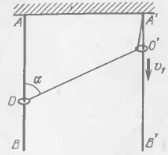
\includegraphics[width=0.9\textwidth]{0113RelativityRings.jpg}
\end{minipage}
\begin{sol}
Перейдем в систему отсчета, связанную с колечком $O'$. В этой системе отсчета скорость точки $O$ равна $v_1/ \cos \alpha$ и направлена вверх, так как нить нерастяжима и относительно колечка $O'$ веревка выбирается с постоянной скоростью $v_1$. Поэтому относительно прямой $АА'$, связанной с землей, скорость колечка $O$ будет равна $v_2 = \frac{v_1}{\cos \alpha} - v_1 = v_1 \frac{\sin^2 (\alpha /2)}{\cos \alpha}$ и направлена вверх.
\end{sol}
\begin{ans}
$v_2 = v_1 \frac{\sin^2 (\alpha /2)}{\cos \alpha}$
\end{ans}
\end{ex}

\begin{ex}
\hspace{0pt} \\
\begin{minipage}{.65\textwidth}
На неподвижном клине, образующем угол $\alpha$  с горизонтом, лежит нерастяжимая невесомая веревка. Один из концов веревки прикреплен к стене в точке $A$. В точке $B$ к веревке прикреплен небольшой грузик. В некоторый момент времени клин начинает двигаться вправо с постоянным ускорением $\vec{a}$. Определите ускорение $\vec{a}_2$ грузика, пока он находится на клине.
\end{minipage}
\begin{minipage}{.35\textwidth}
\centering
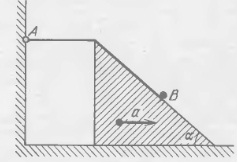
\includegraphics[width=0.9\textwidth]{0114RelativityWedge.jpg}
\end{minipage}
\begin{sol}
К моменту времени $t$ от начала движения клин пройдет расстояние $s = at^2/2$ и приобретет скорость $v_1 = at$. За это время грузик переместится вдоль клина на такое же расстояние $s$, а его скорость относительно клина будет равна $v_2 = at$ и направлена вдоль клина вверх. Скорость грузика относительно земли равна $\vec{v}_3 = \vec{v}_1 + \vec{v}_2$. Поскольку угол между векторами $\vec{v}_1$ и $\vec{v}_2$ равен $\alpha$, то $v_3 = 2at \sin (\alpha /2)$. \\ 
Угол, который скорость $\vec{v}_3$ составляет с горизонтом, равен $\beta  = (\pi - \alpha)/2$. Таким образом, грузик движется вдоль прямой, составляющей с горизонтом угол $\beta$ c ускорением $a_2 = 2a \sin (\alpha /2)$.
\end{sol}
\begin{ans}
Ускорение грузика относительно земли $a_2 = 2a \sin (\alpha /2)$ направлено под углом $\beta  = (\pi - \alpha)/2$ к горизонту.
\end{ans}
\end{ex}

\begin{ex}
\hspace{0pt} \\
\begin{minipage}{.65\textwidth}
(2011) По шоссе со скоростью $\vec{v}_a$ движется автобус. Человек находится на расстоянии $h$ от шоссе и на расстоянии $L$ от автобуса. 
Под каким углом $\alpha$ к шоссе со скоростью $\vec v$  должен идти человек, чтобы выйти на шоссе одновременно с автобусом?
\end{minipage}
\begin{minipage}{.35\textwidth}
\centering
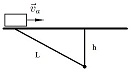
\includegraphics[width=0.9\textwidth]{012011RelativityBus.jpg}
\end{minipage}
\begin{ans}
При $v_a > vL/h$ человек ни при каком угле не сможет оказаться на шоссе раньше автобуса. При $v_a < vL/h$ существует два ответа $\alpha_1 = \arcsin \frac{h}{L} + \arcsin \frac{v_ah}{vL}$ и $\alpha_2 = \pi - \alpha_1$.
\end{ans}
\end{ex}

\begin{ex}
\hspace{0pt} \\
\begin{minipage}{.65\textwidth}
(2007) Два катера вышли одновременно из пунктов $A$ и $B$, находящихся на противоположных берегах реки, и двигались вдоль отрезка $AB$ длины~$l$. 
Прямая $AB$ образует угол $\alpha$ с направлением скорости течения $\vec v$. Скорости движения катеров относительно воды одинаковы. 
На каком расстоянии от пункта $B$ произошла встреча катеров, если они встретились через время $t$ после отхода от причалов?
\end{minipage}
\begin{minipage}{.35\textwidth}
\centering
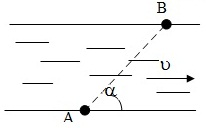
\includegraphics[width=0.9\textwidth]{0115RelativityPowerboats.jpg}
\end{minipage}
\begin{ans}
$l/2 - vt \cos \alpha$
\end{ans}
\end{ex}

\section{Движение тела под углом к горизонту}

\begin{ex} 
Камень брошен с высоты $h$ под углом $\alpha$ к горизонту  со скоростью $v_0$. Какой угол $\beta$ будет составлять скоростью камня с горизонтом в момент падения на землю? Чему равна величина этой скорости? На каком расстоянии $s$ по горизонтали от основания точки запуска упадет камень?
\begin{ans}
$\tan \beta = \sqrt{\tan^2 \alpha + \frac{2gh}{v_0^2 \cos^2 \alpha}}$, $s=\frac{v_0 \cos \alpha}{g} \sqrt{v_0^2 \sin^2 \alpha + 2gh}$.
\end{ans}
\end{ex}

\begin{ex}
Мальчик бросает камень по направлению в кота, сидящего на крае сарая. Через 1 секунду камень падает на землю в точку, находящуюся на одной вертикали с котом. На какой высоте находился кот?
\begin{ans}
$h = g\tau^2/2 = 5$ м		
\end{ans}
\end{ex}	

\begin{ex} 
Мышонок стреляет из рогатки в кота, сидящего на ветке дерева. Через $t = 1$ с камень попадает в ветку прямо у лап кота. На каком расстоянии $s$ от мышонка находился кот, если известно, что векторы $\vec v(0)$ и $\vec v(t)$ взаимно перпендикулярны? 
Ускорение свободного падения $g$ = 10 м/с\textsuperscript{2}. Сопротивление воздуха пренебрежимо мало.
\begin{ans}
$h = gt^2/2 = 5$ м
\end{ans}
\end{ex}

\begin{ex}
Камень бросили с горизонтальной площадки под углом к горизонту в направлении вертикальной стены. Камень упруго ударился о стену и упал на площадку. Известно, что время полёта от момента бросания до удара составило $t_1$, а время полёта от удара до падения $t_2$. Определите, на какой высоте камень ударился о стену. Стена перпендикулярна плоскости, в которой движется камень. Влиянием воздуха можно пренебречь.
\begin{ans}
$h = gt_1t_2/2$
\end{ans}
\end{ex}

\begin{ex}
Маленький шарик, брошенный с начальной скоростью $\vec{v}_0$ под углом $\alpha$ к горизонту, 
ударился о вертикальную стенку, движущуюся ему навстречу с горизонтально направленной скоростью $\vec u$, и отскочил в точку, из которой был брошен. 
Определите, через какое время $t_1$ после броска произошло столкновение шарика со стенкой? Потерями на трение пренебречь.
\begin{sol}
Пусть время движения от соударения до возвращения в точку бросания равно $t_2$. Поскольку при упругом ударе вертикальная составляющая скорости не меняется, а горизонтальная скорость увеличивается до величины $v_0 \cos \alpha + 2u$, то полное время полета составит $t_1 + t_2 = \frac{2v_0 \sin \alpha}{g}$. Расстояние по горизонтали от места броска до места удара о стенку выражается в виде $v_0 \cos \alpha t_1 = (v_0 \cos \alpha +2u)t_2$, откуда $t_1 = \frac{v_0 \sin \alpha (v_0 \cos \alpha + 2u)}{g(v_0 \cos \alpha + u)}$.
\end{sol}
\begin{ans}
$t_1 = \frac{v_0 \sin \alpha (v_0 \cos \alpha + 2u)}{g(v_0 \cos \alpha + u)}$
\end{ans}
\end{ex}

\begin{ex}
С какой минимальной скоростью можно перебросить камень через здание высоты $H$ с куполообразной крышей радиуса $R$?
\begin{ans}
$v_{min} = \sqrt{g(R+2H)}$
\end{ans}
\end{ex}

\begin{ex}
Зенитное орудие может сообщить снаряду начальную скорость $v_0$ в любом направлении. Требуется найти зону поражения, т.е. границу отделяющую цели, до которых снаряд из данного орудия может долететь, от недостижимых целей. Сопротивлением воздуха пренебречь. 
\begin{ans}
$y = \frac{v_0^2}{2g} - \frac{gx^2}{2v_0^2}$
\end{ans}
\end{ex}

\begin{ex}
В спортивном зале высотой $h$ бросают маленький мяч с начальной скоростью $v_0$. Определите, какое максимальное расстояние по горизонтали может пролететь мяч после бросания до первого удара о пол, если соударение с потолком абсолютно упругое. Считайте, что мяч бросают с уровня пола. Пол и потолок горизонтальны, сопротивление воздуха пренебрежимо мало.
\begin{ans}
Если $v_0 < 2 \sqrt{gh}$, то дальность полета $L = \frac{v_0^2}{g}$; если $v_0 > 2 \sqrt{gh}$, то $L = 4h \sqrt{\frac{v_0^2}{2gh}-1}$.
\end{ans}
\end{ex}

\begin{ex}
Необходимо с поверхности земли попасть камнем в цель, расположенную на расстоянии $L$ по горизонтали на высоте $H$. С какой наименьшей скоростью это можно сделать? Трением пренебречь.
\begin{ans}
$v_{min} = \sqrt{g \left(\sqrt{l^2 + h^2} + h \right)}$
\end{ans}
\end{ex}

\begin{ex}
(2004) При какой минимальной начальной скорости $v_0$ можно перебросить камень через дом с покатой крышей? 
Ближайшая стена имеет высоту $H$, задняя стена -- высоту $h$, ширина дома равна $l$.
\begin{center}
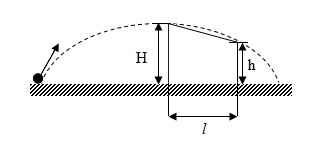
\includegraphics[width=5.0cm]{0209AngleHouse.jpg}
\end{center}
\begin{sol}
Требование минимальности скорости бросания камня с поверхности земли означает, что оптимальная траектория камня пройдет через точки "вершины" крыши В и С, расположенные на высотах $H$ и $h$ соответственно. Обратим движение камня и определим минимальную скорость в точке C -- $v_C$, при которой камень может перелететь через точку В. Учитывая решение предыдущей задачи, легко понять, что $v_B = \sqrt{g \left(\sqrt{l^2 + (H-h)^2} + H-h \right)}$. Минимально возможную скорость бросания камня с земли $v_{min}$ найдем из закона сохранения энергии $v_{min}^2 = v_B^2 + 2gH$, откуда $v_{min} = \sqrt{g \left(\sqrt{l^2 + (H-h)^2} + H + h \right)}$.
\end{sol}
\begin{ans}
$v_{min} = \sqrt{g \left(\sqrt{l^2 + (H-h)^2} + H + h \right)}$
\end{ans}
\end{ex}

\begin{ex}
(2018) Тело бросают с поверхности длинной наклонной плоскости. Угол наклона плоскости к горизонту $\alpha = 45^{\circ}$, величина начальной скорости фиксирована. 1) Под каким углом к горизонту нужно бросить тело для того, чтобы время полета было максимально? 2) Под каким углом к горизонту нужно бросить тело для достижения максимальной дальности (дальность откладывается вдоль плоскости)?
\begin{ans}
1) $\pi/2$; 2) $\pi/8$
\end{ans}
\end{ex}

\begin{ex}
(2005) Колесо радиуса $R$ катится по горизонтальной мокрой дороге со скоростью $v$. 1) На какую максимальную высоту $h$ поднимаются капли воды, отрывающиеся от колеса? 2) Какой должна быть минимальная скорость колеса, чтобы капелька, достигшая максимальной высоты, опустилась на то же самое место? 3) Изменится ли высота $h$, если колесо будет катиться с пробуксовкой?
\begin{ans}
1) При $gR > v^2$ максимальная высота подъема $h = 2R$, при $gR < v^2$ -- $h = R +\frac{v^2}{2g} + \frac{gR^2}{2v^2}$; 2) $v_{min} = \frac{\pi g R}{(1+ \sin \alpha) \cos \alpha}$, где $\sin \alpha = gR/v^2$; 3) изменится.
\end{ans}
\end{ex}

\begin{ex}
(2010) В сферической лунке прыгает шарик, упруго отражаясь от ее стенки в двух точках, расположенных на одной горизонтали. Промежуток времени при движении шарика слева направо равен $T_{1}$, а при движении справа налево -- $T_2$. Определите радиус лунки.
\begin{ans}
$R = \sqrt{g} T_1 T_2 /2\sqrt{2}$
\end{ans}
\end{ex}

\begin{ex}
Из точек A и В, находящихся на одной горизонтальной прямой, одновременно бросили два камня с одинаковыми по модулю скоростями $v_0$ = 20 м/с. 
Один из камней полетел по навесной траектории, другой -- по настильной, но каждый попал в точку старта другого камня. 
Известно, что в точке А угол бросания $\alpha = 75^{\circ}$. 
Через какое время $\tau$ после старта расстояние между камнями станет минимальным? Чему равно это расстояние?
\begin{ans}
$s = 10$ м, $\tau = v_0 \sin 150^{\circ} \cos 30^{\circ} \cos 45^{\circ} /g$
\end{ans}
\end{ex}

\begin{ex}
Две частицы одновременно начали двигаться в однородном поле тяжести $\vec g$. Начальные их скорости равны по модулю $v_0$ и лежат в одной вертикальной плоскости. Угол наклона вектора одной из скоростей к горизонту равен $\alpha$, а другой $2\alpha$. В какой момент времени $\tau$ от начала движения скорости частиц окажутся сонаправленными? Сопротивлением движению пренебречь.
\begin{ans}
$\tau = \frac{v_0 \cos (\alpha /2)}{g \sin (3\alpha / 2)}$
\end{ans}
\end{ex}

\begin{ex}
(1998) Шарик, которому сообщена горизонтальная скорость $v$, падает на горизонтальную плиту с высоты $h$. При каждом ударе о плиту вертикальная составляющая скорости уменьшается (отношение вертикальной составляющей скорости после удара к ее значению до удара постоянно и равно $\alpha$). Определить, на каком расстоянии $х$ от места бросания отскоки шарика прекратятся. Считать, что трение отсутствует, так что горизонтальная составляющая скорости шарика $v$ не меняется.
\begin{ans}
$x = v \sqrt{2h/g} \left( 1 + \alpha \right) / \left( 1 - \alpha \right)$
\end{ans}
\end{ex}
\section{Мгновенный центр вращения}
%TODO задача про солнечный зайчик, скорость которо превышает скорость света

\begin{ex}
Колесо радиуса $R$ катится без проскальзывания по горизонтальной поверхности со скоростью $v$. 
Найдите скорости различных точек колеса, уравнения траектории и радиус кривизны траектории в верхней точке дуги для произвольной точки на ободе колеса.
\begin{ans}
$v(\varphi) = v\sqrt{2(1- \cos \varphi)}$, $x(t) = vt - R \sin \varphi$, $y(t) = R(1 - \cos \varphi)$, $\varphi = vt / R$, $R_k = 4R$.
\end{ans}
\end{ex}

\begin{ex}
Скорость одного конца стержня равна $v$ и направлена под углом $\alpha$ к стержню. Найдите скорость другого конца, которая направлена под углом $\beta$ к стержню.
\begin{ans}
$u = v \cos \alpha / \cos \beta$
\end{ans}
\end{ex}

\begin{ex}
По гладкому горизонтальному столу свободно скользит тонкая прямая однородная палочка длины $L$. 
В некоторый момент скорость одного из концов равна $v$ и составляет прямой угол с палочкой, 
а скорость другого конца по величине равна $2v$. За какое время палочка повернется на угол $2\pi$?
\begin{ans}
$T_1 = 2 \pi L/v$, $T_2 = 2 \pi L/3v$.
\end{ans}
\end{ex}

\begin{ex}
\hspace{0pt} \\
\begin{minipage}{.65\textwidth}
(2006) Между двумя стенками, образующими прямой угол, движется по направляющим без отрыва стержень $AB$ длиной $l_0$. 
Скорость точки $B$ постоянна, равна $v_0$ и направлена горизонтально. Определить скорость $v$ и ускорение $a$ точки $M$, расположенной на расстоянии $MB$ = $l$ от точки $B$, в момент времени, когда угол между горизонтальной стенкой и стержнем $AB$ составляет $\alpha$.
\end{minipage}
\begin{minipage}{.35\textwidth}
\centering
\includestandalone[width=0.9\textwidth]{Pictures/032006RotationKinematicsBar}
\end{minipage}
\begin{ans}
$\omega = v_0/l_0 \sin \alpha$, $R = sqrt{l^2 + l_0^2 - 2ll_0 \sin \alpha}$, $v_M = \omega R$.
\end{ans}
\end{ex}

\section{Бесконечно малые перемещения}

\begin{ex}
Тело движется по окружности радиуса $R$ так, что его скорость зависит от времени по линейному закону: $v = at$. Найдите зависимость ускорения тела от времени.
\begin{ans}
$a_p = \sqrt{a^2 + a^4t^4/R^2}$
\end{ans}
\end{ex}

\begin{ex}
\hspace{0pt} \\
\begin{minipage}{.65\textwidth}
Луч света падает на вращающийся экран $AO$, образуя на нем зайчик $C$. Угловая скорость вращения экрана $\omega$\,; угол, образуемый лучом света с горизонтом, равен $\alpha$. В некоторый момент времени экран занимает положение, изображенное на рисунке, при этом расстояние от оси вращения до зайчика $OC$ = $l$. Определите, какую скорость имеет зайчик относительно экрана в указанный момент времени.
\end{minipage}
\begin{minipage}{.35\textwidth}
\centering
\includestandalone[width = 0.9\textwidth]{Pictures/0307InfinitesimalChangeRay}
\end{minipage}
\begin{ans}
$v = \omega l \tan \alpha$
\end{ans}
\end{ex}

\begin{ex}
\hspace{0pt} \\
\begin{minipage}{.65\textwidth}
Определить скорость точки пересечения двух лучей прожекторов, которые вращаются в противоположных направлениях с угловой скоростью $\omega$, в момент, когда угол наклона к горизонту обоих прожекторов равен $\varphi$. Расстояние между прожекторами равно $2l$.
\end{minipage}
\begin{minipage}{.35\textwidth}
\centering
\includestandalone[width = 0.9\textwidth]{Pictures/0308RotationKinematicsProjectors}
\end{minipage}
\begin{ans}
$v = \omega l/ \cos^2 \varphi$
\end{ans}
\end{ex}

\begin{ex}
\hspace{0pt} \\
\begin{minipage}{.65\textwidth}
Бревно, упираясь одним концом в угол между землей и стеной, касается грузовика на высоте $h$, который отъезжает от стены со скоростью $u$. Как зависит угловая скорость вращения бревна от угла $\alpha$ между бревном и горизонтом?
\end{minipage}
\begin{minipage}{.35\textwidth}
\centering
\includestandalone[width = 0.9\textwidth]{Pictures/0309RotationKinematicsLorry}
\end{minipage}
\begin{ans}
$\omega = u \sin^2 \alpha /h$
\end{ans}
\end{ex}

\begin{ex}
За лисой, бегущей прямолинейно с постоянной скоростью $v$, бежит собака таким образом, что ее скорость $u$ всегда направлена на местоположение лисы. В момент, когда векторы скоростей перпендикулярны, расстояние между ними было равно $L$. С каким ускорением при этом двигалась собака?
\begin{ans}
$a = uv/L$
\end{ans}
\end{ex}

\begin{ex} 
\hspace{0pt} \\
\begin{minipage}{.65\textwidth}
На диск радиуса $R$ намотаны две нерастяжимые нити, закрепленные в двух разных точках. При отпускании диск вращается. Когда угол между нитями у диска $\alpha$, угловая скорость вращения диска $\omega$. С какой скоростью в этот момент движется центр диска? Нити остаются натянутыми.
\end{minipage}
\begin{minipage}{.35\textwidth}
\centering
\includestandalone[width = 0.9\textwidth]{Pictures/0311RotationKinematicsDisc}
\end{minipage}
\begin{ans}
$\omega R/ \cos (\alpha /2)$
\end{ans}
\end{ex}

\begin{ex}
Внутри неподвижной окружности катится без скольжения другая окружность вдвое меньшего радиуса. Какую траекторию описывает при этом произвольно выбранная точка на подвижной окружности?
\begin{ans}
отрезок
\end{ans}
\end{ex}

\begin{ex}
\hspace{0pt} \\
\begin{minipage}{.65\textwidth}
Бусинка может двигаться по кольцу радиуса $R$, подталкиваемая спицей, которая вращается с угловой скоростью $\omega$ в плоскости кольца. Ось вращения спицы находится на кольце. Определить ускорение бусинки.
\end{minipage}
\begin{minipage}{.35\textwidth}
\centering
\includestandalone{Pictures/0313RotationKinematicsRingAndBead}
\end{minipage}
\begin{ans}
$4 \omega^2 R$
\end{ans}
\end{ex}

\begin{ex}
По палочке, которая вращается с угловой скоростью $\omega$, ползет жук со скоростью $v$. Определите скорость и ускорение жука, когда он находится на расстоянии $L$ от оси вращения палочки.
\begin{ans}
$u = \sqrt{v^2 + \omega^2 L^2}$, $a = \sqrt{\omega^4 L^2 + 4\omega^2 v^2}$
\end{ans}
\end{ex}

\begin{ex}
(2003) Четыре черепахи находятся в вершинах квадрата со стороной $l$. Они начинают двигаться одновременно с постоянной скоростью $v$. Каждая черепаха движется по направлению к своей соседке по часовой стрелке. Где встретятся черепахи и через какое время? Найти угол между скоростью движения черепахи и одной из сторон квадрата как функцию ее координат $\varphi = \varphi (x,y)$.
\begin{ans}
В центре через $t = v/l$, $\tan \alpha = (x-y)/(x+y)$.
\end{ans}
\end{ex}
\section{Динамика}
%TODO Добавить задачи на системы блоков + задачи Черепанова
 
\begin{ex}
На наклонной поверхности с углом $\alpha$ к горизонту находится брусок. 
Коэффициент трения бруска о поверхность равен $\mu$. С каким ускорением будет двигаться брусок?
\begin{ans}
если $\mu > \tan \alpha$, то $a = 0$; если $\mu < \tan \alpha$, то $a = g(\sin \alpha - \mu \cos \alpha)$.
\end{ans}
\end{ex}

\begin{ex}
\hspace{0pt} \\
\begin{minipage}{.65\textwidth}
(2005) Между двумя неподвижными муфтами может без трения перемещаться вверх и вниз стержень, масса которого $m$. Стержень нижним концом касается гладкой поверхности клина массой $M$. Клин лежит на гладком горизонтальном столе. Определите ускорения стержня и клина.
\end{minipage}
\begin{minipage}{.35\textwidth}
\centering
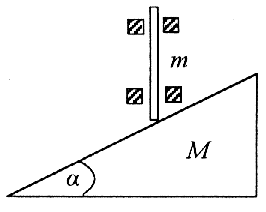
\includegraphics[width = 0.9 \textwidth]{ConnectedInclinedRod.png}
\end{minipage}
\begin{ans}
$a_1 = g \frac{m \sin^2 \alpha}{m \sin^2 \alpha + M \cos^2 \alpha}$, $a_2 = g\frac{m \sin \alpha \cos \alpha}{m \sin^2 \alpha + M \cos^2 \alpha}$
\end{ans}
\end{ex}

\begin{ex}
Клин высотой $h$ с углом наклона $\alpha$ стоит на гладкой горизонтальной поверхности. Масса клина $m_1$. С вершины клина начинает соскальзывать без трения брусок массой $m_2$. Найдите ускорение клина и время соскальзывания бруска.
\begin{ans}
$a_1 = g \frac{m_2 \sin \alpha \cos \alpha}{m_1 + m_2 \sin^2 \alpha}$, $t=\sqrt{\frac{2h(m_1+m_2\sin^2\alpha)}{(m_1+m_2)g \sin^2 \alpha}}$
\end{ans}
\end{ex}

\begin{ex}
(2015) Брусок скользит по длинной наклонной плоскости с углом наклона $\alpha = 30^{\circ}$, движущейся равномерно относительно земли по горизонтальной поверхности со скоростью $u = 10$ м/с в направлении противоположном вершине с углом $\alpha$. Начальная скорость бруска относительно плоскости равна нулю, коэффициент трения бруска о плоскость $\mu = 0,4$. 1) Определите минимальную скорость бруска относительно земли. 2) Через какое время скорость бруска относительно земли будет равна 10 м/с? 3) По какой траектории будет двигаться брусок относительно земли?
\begin{ans}
$v_{min} = u \sin \alpha = 5$ м/c, $t = v_2/g(\sin \alpha - \mu \cos \alpha) = 11,3$ с, парабола.
\end{ans}
\end{ex}

\begin{ex}
\hspace{0pt} \\
\begin{minipage}{.65\textwidth}
Брусок массы $m$ тянут за нить так, что он движется с постоянной скоростью по
горизонтальной плоскости с коэффициентом трения $\mu$. Найти угол $\alpha$, при котором натяжение нити минимально. Чему оно равно?
\end{minipage}
\begin{minipage}{.35\textwidth}
\centering
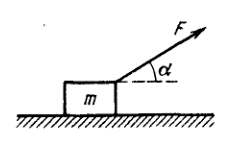
\includegraphics[width = 0.9 \textwidth]{MinForceAngle.png}
\end{minipage}
\begin{ans}
$\tan \alpha = \mu$, $F = \mu mg / \sqrt{\mu^2 + 1}$
\end{ans}
\end{ex}

\begin{ex}
По наклонной плоскости, образующей угол $\alpha$ с горизонтом, за веревку вытягивают ящик массы $m$. 
Коэффициент трения ящика о плоскость равен $\mu$. Под каким углом $\beta$ к горизонту следует тянуть веревку, 
чтобы равномерно двигать ящик с наименьшим усилием? Каково это усилие?
\begin{ans}
$\tan \beta = \mu$, $F = mg \sin (\alpha + \beta)$ при $\alpha + \ beta < \pi/2$, иначе $F = mg$.
\end{ans}
\end{ex}

\begin{ex}
(2016) Брусок массой 10 кг положили на наклонную плоскость с углом наклона к горизонту $\alpha = 30^{\circ}$. Коэффициент трения между бруском и плоскостью равен $\mu = 0,8$. 1) Докажите, что брусок будет покоиться относительно плоскости. 2) Определите минимальную горизонтальную силу, направленную вдоль наклонной плоскости и перпендикулярно плоскости рисунка, которую нужно приложить к бруску, чтобы его сдвинуть. 3) Определите минимальную силу‚ которую нужно приложить к бруску для того, чтобы перемещать его вверх по наклонной плоскости.
\begin{center}
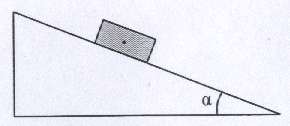
\includegraphics[width = 0.4\textwidth]{InclinedSurfaceFriction.png}
\end{center}
\begin{ans}
$F_2 = mg \sqrt{(\mu \cos \alpha)^2 - (\sin \alpha)^2} = 48$ Н, $F_3 = mg(\mu \cos \alpha + \sin \alpha)/\sqrt{\mu^2 + 1} = 93,1$ Н. 
\end{ans}
\end{ex}

\begin{ex}
\hspace{0pt} \\
\begin{minipage}{.65\textwidth}
При какой максимальной силе $F$ верхний брусок еще не будет скользить по нижнему? Массы брусков $m_1$ и $m_2$, коэффициент трения между ними $\mu$, поверхность стола гладкая.
\end{minipage}
\begin{minipage}{.35\textwidth}
\centering
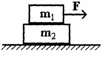
\includegraphics{0403DynamicsBlocks.jpg}
\end{minipage}
\begin{ans}
$F = \mu m_1 g \left(m_1/m_2 + 1 \right)$
\end{ans}
\end{ex}

\begin{ex}
\hspace{0pt} \\
\begin{minipage}{.65\textwidth}
Листы бумаги, сложенные, как показано на рисунке, склеивают свободными концами через лист таким образом, что получаются две самостоятельные кипы $A$ и $B$. Вес каждого листа 0.06 Н, число всех листов 200, коэффициент трения бумаги о бумагу, а также о стол, на котором бумага лежит, равен 0.2. Предполагая, что одна из кип удерживается неподвижно, определить наименьшее горизонтальное усилие $F$, необходимое для того, чтобы вытащить вторую кипу.
\end{minipage}
\begin{minipage}{.35\textwidth}
\centering
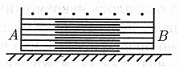
\includegraphics[width = 0.9 \textwidth]{0402DynamicsPaper.jpg}
\end{minipage}
\begin{ans}
$F = 20100 \mu mg = 241,2$ Н
\end{ans}
\end{ex}

\begin{ex}
\hspace{0pt} \\
\begin{minipage}{.65\textwidth}
По вертикально подвешенному в поле тяжести Земли кольцу радиуса $R$ может скользить без трения шарик массы $m$. 
В начальный момент времени кольцо неподвижно, и шарик находится в нижней точке кольца. 
Как будет двигаться шарик, если кольцо начнет вращаться вокруг вертикальной оси с угловой скоростью $\omega$?
\end{minipage}
\begin{minipage}{.35\textwidth}
\centering
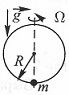
\includegraphics{0405DynamicsRing.jpg}
\end{minipage}
\begin{ans}
$\cos \alpha = g/\omega^2 R$, при $g < \omega^2 R$, иначе $\alpha = 0$.
\end{ans}
\end{ex}

\begin{ex}
\hspace{0pt} \\
\begin{minipage}{.65\textwidth}
К вершине прямого кругового конуса с помощью нити длиной $L$ прикреплена небольшая шайба. Вся система вращается вокруг оси конуса, расположенной вертикально. При каком числе оборотов в единицу времени шайба не будет отрываться от поверхности конуса? Угол при вершине конуса $2\alpha$.
\end{minipage}
\begin{minipage}{.35\textwidth}
\centering
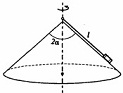
\includegraphics{0406DynamicsCone.jpg}
\end{minipage}
\begin{ans}
$\nu = \frac{1}{2\pi}\sqrt{\frac{g}{L \cos \alpha}}$
\end{ans}
\end{ex}

\begin{ex}
У края диска радиусом $R$ лежит монета. Диск раскручивается так, что его угловая скорость линейно растет со временем по закону $\omega = \varepsilon t$.  В какой момент времени монета слетит с диска, если коэффициент трения между диском и монетой равен $\mu$? Какой угол с направлением к центру диска образует сила трения в этот момент?
\begin{ans}
При $\varepsilon < \mu g /R$ $t=\frac{1}{\sqrt{\varepsilon}}\left( \frac{\mu^2 g^2}{\varepsilon^2 R^2} - 1 \right)^{\frac{1}{4}}$, $\tan \alpha = \left( \frac{\mu^2 g^2}{\varepsilon^2 R^2} - 1 \right)^{-\frac{1}{24}}$
\end{ans}
\end{ex}

\begin{ex}
\hspace{0pt} \\
(2017) На рисунке представлен горизонтальный пружинный маятник, который может совершать колебания с частотой 2 Гц. Масса груза маятника 100 г. Горизонтальная плоскость гладкая. На маятник, находящийся в состоянии покоя в положении равновесия, начинает действовать постоянная горизонтальная сила $F = 2$ Н. 1) Определите максимальное растяжение пружины. 2) Определите максимальное растяжение пружины при условии, что сила $F$ действует только в течение времени 0,01 с.
\begin{center}
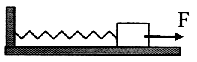
\includegraphics[width = 0.4 \textwidth]{ForceSpring.png}
\end{center}
\begin{ans}
$x = \frac{2F}{4\pi^2 \nu^2 m} = 25,3$ см, $x = v\sqrt{\frac{m}{k}}=15,9$ мм
\end{ans}
\end{ex}
\section{����� ����}

%1
\AddProb ������ ���������� �������� ������ $l$ � ������ $m$ ������� � �������� ����� ������� �������������� ����������� ���, 
��� �� �������� ������������� � ������������ ��������� � ������� ��������� $\omega$ ������ ��� ���������������� ������� � ���������� ����� ��� �����. 
������� ��������� ������� � ����������� �� ���������� $x$ �� ��� ������.

\AddProb ������� ������ ������� �� ���� �����-����������� ������� $m_1$ � $m_2$, 
���������� ����� �������� �� �������� � �������� ������ $L$. ������� ������ �������� ������� ������.

\AddProb ��� �������� ����� $m$ � $2m$ ������� ��������� ����� ������ $l$ � �������� �� ������� �������������� ���������. 
� ��������� ������ ������� �������� ����� $2m$ ����� ����, � �������� ����� $m$ ����� $v$ � ���������� ��������������� ����. 
������� ��������� ���� � ������ �������� �������.

\AddProb (1998) �� ������� �������������� ��������� ����� ��� ���������� ������ ������ $m$ ������, 
��������� ������ �������� ���������� $k$. ������� ������ �������� �������� $v_0$ � ����������� �� ������� ������. 
������� �������� �������. ����� ����� ����� ���������� ������� ������� ��������� ������������� ��������? 

\begin{figure}[!h]
\centering
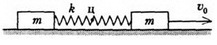
\includegraphics{051998CenterOfMassSpring.jpg}
\end{figure}

\AddProb ��� ������ $m$ �������� �� ��������� $v$ �� ���������� ��� ������ $2m$. 
������� �������� ����� ����� ����� �������� ������������ �����. 

%6
\AddProb ����������, ����� ����� ����� ������������ ������� ������ ������� ������ $m_1$ ��� ������� ������� ������������ 
� ����������� �������� ������ $m_2$. 

\AddProb ��������, ��� ��� ������� ������������� ����� ���� ���������� �����, ���� �� ������� �� ����� ��������, 
���� ������� ����� $90^{\circ}$. �������� ��� �����������.

\AddProb (2009) ��������� �������� ����� $L$ � ����� �������� �� ������ � ������� $m$ � $3m$ ��������� �� ������� �������������� ���������. 
������ ������ $m$ ����� �������� �������� $v$ � �����������, ���������������� �������. ������ ���� ��������� �������? 
��� ��������� �����, ���� �������� $v$ �������� ������ ������ $3m$? ����� ����� ������� �������� � ������������ ������� ������������� �������� � ������ � ������ �������?

\AddProb (2012) �� ��������� ������� ����� ����� ����� ������ $M$ � �������� $R$. �� ������ ��������� ���, ����� �������� $m$. 
����� ���������� ����� ��������� ��� � ����� ������ ��� �������� ���� �� ������?

\begin{wrapfigure}{r}{5.5cm}
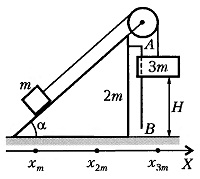
\includegraphics{0510CenterOfMassWedge.jpg}
\end{wrapfigure}

\AddProb ���� ������ $2m$ � ����� ������� � ��������� $\alpha $ ($\cos~\alpha$~=~2/3) ��������� �� ������� �������������� ����������� �����. 
����� ����, ����������� �� ������� �����, ���������� ������ ����, ����������� ����� ������� $m$ � $3m$. 
���� ������ $3m$ ����� ��������� ����� ������������ ������������ ��, ������������ �� �����. 
���� ���� ������� ���������� ���������� �� ���������� $H$~=~27~�� �� �����, � ����� ���������. 
�� ����� ���������� ��������� ���� � ������� ������� ����� ������ $3m$ �����? ������� ����� � ������������ �� ����������.


\section{�������������� �����}

%11
\AddProb ����� ���� �������� $S$ ��������� � ������, ������������� ��������������� �����. 
�������� ���� � ����� $v$, ����� ����� ���� ������ �������� � ������� �� ������. ������ ���� �������� ���� �� ������? ��������� ���� $\rho$.

\AddProb ����������� ������� ������ $M$ �������� � �������� �������. ��� ���������� �������� ������������ ���������� ���������, 
������� ����������� ���������� ����� �� ��������� $u$ ������������ �������, ������ ������ ������� � ����� ����� $\mu$ 
(������ ������� -- ��� ����� �������, ������������� �� ������� �������). ������� ��������� �������.

\begin{wrapfigure}{r}{2.5cm}
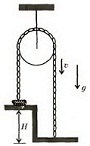
\includegraphics{0503DistributedMassChainAndPulley.jpg}
\end{wrapfigure}

\AddProb ������� ������ ������� ���������� ����� ���� ���, ��� �� ������ ����� ������� �� ����, � ����� �����, 
����������� �������, �� ������ ������� $H$. ������� ���������, � ��� �������� � ��������. 
������� �������������� �������� �������� �������. ���� ���������, ������� ���������.

\AddProb ������ ���������� ������ ������ $m$ � �������� $R$ �������� �� ������� �������������� ����������� � 
���������� �� ������� �������� $\omega$. ������� ���� ��������� �������.

\begin{figure}[!h]
	\begin{subfigure}{.3\textwidth}
		\centering
		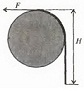
\includegraphics{0505DistributedMassRope.jpg}
	\end{subfigure}		
	\begin{subfigure}{.7\textwidth}
		\centering
		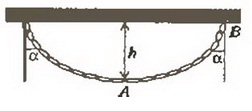
\includegraphics{0506DistributedMassChainAndCeiling.jpg}
	\end{subfigure}		
\end{figure}

\AddProb ������� ������ $l$ � ������ $m$ ������ �� ������� �������������� ������ �������� $R$, 
������ ������� ������� ���������� �� ������� �����, ����������� �������������� ���� $F$, � ����� ���������. 
����������: 1) �������� ���� $F$; 2) ��������� ������� � ������ ������.

%16
\AddProb ������� ������ $m$ � ������ $l$ ��������� �� ����� � �������. 
��� ���� ���������, ��� � ������ ����������� ������� �������� ���� $\alpha $ � ����������. 
������� ���������� $h$ �� ������ ����� ������� �� �������.

\begin{wrapfigure}{r}{3.5cm}
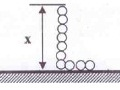
\includegraphics{0507DistributedMassChainAndTable.jpg}
\end{wrapfigure}

\AddProb (2011) ���������� ������� ������ $L$ � ������ $m$ ��������� �� ���� ���, ��� ������ ������ ��� �������� �����. 
���� ����������. ����� ����������� ���� �������� $F$ ������� �� ���� �� ����� $x$ ��� �� ������� �����. ������� ���� ������� � ���� ���������.
\section{Теорема об изменении механической энергии}

\begin{ex}
\hspace{0pt} \\
\begin{minipage}{.65\textwidth}
На бруске длиной $l$ массой $M$, расположенном на гладкой горизонтальной поверхности, лежит маленькое тело массой $m$. Коэффициент трения между телом и бруском $\mu$. С какой скоростью $v$ должна двигаться система, чтобы после упругого удара бруска о стенку тело упало с бруска?
\end{minipage}
\begin{minipage}{.35\textwidth}
\centering
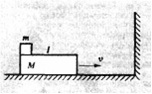
\includegraphics[width = 0.9 \textwidth]{0601MechanicalEnergyBlocks.jpg}
\end{minipage}
\begin{ans}
$v > \sqrt{\mu g l(1+m/M)/2}$
\end{ans}
\end{ex}

\begin{ex}
\hspace{0pt} \\
\begin{minipage}{.65\textwidth}
Тело массой $m$ съезжает с высоты $h$ гладкой наклонной плоскости и начинает скользить по тележке массой $M$, находящейся на гладкой горизонтальной поверхности. Коэффициент трения между телом и тележкой $\mu$. На какое расстояние переместится тело относительно тележки?
\end{minipage}
\begin{minipage}{.35\textwidth}
\centering
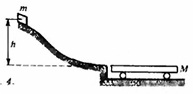
\includegraphics[width = 0.9 \textwidth]{0602MechanicalEnergyHill.jpg}
\end{minipage}
\begin{ans}
$L = hM/\mu(m+M)$
\end{ans}
\end{ex}

\begin{ex}
\hspace{0pt} \\
\begin{minipage}{.65\textwidth}
На горизонтальной плоскости лежит тело массой $m$, соединенное с вертикальной стеной пружиной жесткостью $k$. В начальный момент времени пружина не деформирована. На тело начинает действовать постоянная сила $F$. Считая, что коэффициент трения между телом и плоскостью $\mu$ и что $F >\mu mg$, найдите максимальное смещение тела от начального положения и максимальную скорость тела в процессе движения.
\end{minipage}
\begin{minipage}{.35\textwidth}
\centering
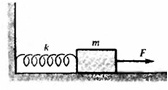
\includegraphics[width = 0.9 \textwidth]{0603MechanicalEnergySpring.jpg}
\end{minipage}
\begin{ans}
$x_m = 2(F-\mu mg)/k$, $v_m = \sqrt{\frac{k}{m}}\frac{F-\mu mg}{k}$
\end{ans}
\end{ex}

\begin{ex}
\hspace{0pt} \\
\begin{minipage}{.65\textwidth}
Груз массой $m$ медленно поднимают на высоту $h$ по наклонной плоскости с помощью блока и троса. 
При этом совершается работа $A$. Затем трос отпускают, и груз скользит вниз. Найдите величину $A$, если известно, 
что скорость тела в конце спуска равна $v$.
\end{minipage}
\begin{minipage}{.35\textwidth}
\centering
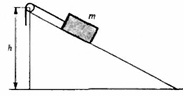
\includegraphics[width = 0.9 \textwidth]{0604MechanicalEnergyWedgeAndBlock.jpg}
\end{minipage}
\begin{ans}
$A=2mgh - mv^2/2$
\end{ans}
\end{ex}

\begin{ex}
(2010) У основания наклонной плоскости находится брусок. Бруску сообщают некоторую начальную скорость, 
направленную вдоль плоскости вверх. На высоте $h$ скорость бруска уменьшается до значения $v_1$. 
После абсолютно упругого удара о стенку, расположенную на высоте $H > h$, брусок скользит вниз, 
и на той же высоте $h$ его скорость равна $v_2<v_1$. Определите скорость бруска в момент удара о стенку.
\begin{ans}
$v^2 = (v_1^2 + v_2^2)/2 - g(H-h)$
\end{ans}
\end{ex}

\section{Энергия и импульс}

\begin{ex}
На гладкой горизонтальной поверхности лежит небольшая шайба массы $m$ и гладкая горка массы $M$ высоты $H$. Какую минимальную скорость $v$ надо придать шайбе, чтобы она смогла преодолеть барьер?
\begin{ans}
$v = \sqrt{2gH(1+m/M)}$
\end{ans}
\end{ex}

\begin{ex}
(2012) Две лодки идут параллельными курсами навстречу друг другу с одинаковыми скоростями $v$. Когда лодки встречаются, с одной лодки на другую перебрасывают груз массой $m$, а затем со второй лодки на первую перебрасывают такой же груз. 
В другой раз грузы перебрасывают из лодки в лодку одновременно. В каком случае скорости лодок после перебрасывания грузов будут больше? 
Масса каждой лодки без груза $M$.
\begin{ans}
$v_1 = Mv/(M+2m) > v_2 = v(M-m)/(M+m)$
\end{ans}
\end{ex}

\begin{ex}
(2006) Лягушка массы $m$ сидит на конце доски массы $M$ и длины $L$. Доска плавает по поверхности пруда. Лягушка прыгает под углом $\alpha$ к горизонту вдоль доски. Какой должна быть начальная скорость лягушки, чтобы она оказалась после прыжка на противоположном конце доски? Как изменится ответ, если 1) доска и лягушка сносятся течением со скоростью $u$, и лягушка прыгает по направлению против течения; 2) доска испытывает при своем движении постоянную силу сопротивления воды $F$?
\begin{ans}
$v_0 = \sqrt{\frac{gLM}{(M-m) \sin 2\alpha}}$
\end{ans}
\end{ex}

\begin{ex}
(2001) Трактор массы $m$ рывками перемещает груз массы $M>m$. Они соединены прочным нерастяжимым тросом длины $L$. В начальный момент трактор находится рядом с грузом. Сколько рывков надо сделать трактору, чтобы переместить его на расстояние $s$?  Считать, что коэффициент трения трактора и груза о землю одинаков.
\begin{ans}
$N = s(M-m)/L(M+m)$
\end{ans}
\end{ex}

\begin{ex}
Два груза массы $m$, соединенные пружиной жесткостью $k$, находятся на гладком горизонтальном столе. Одному из тел сообщают скорость $v$ и измеряют максимальное растяжение пружины. В ходе опыта пружина лопнула при растяжении, равном половине максимального. С какими скоростями после разрыва пружины грузы поедут по столу?
\begin{ans}
$v_{1,2} = (2\pm \sqrt{3})/4$
\end{ans}
\end{ex}

\begin{ex}
\hspace{0pt} \\
\begin{minipage}{.65\textwidth}
Два тела малых размеров массой $m$ каждое соединены стержнем пренебрежимо малой массы длиной $l$. Система из начального положения у вертикальной гладкой стены приходит в движение. Нижнее тело скользит без трения по горизонтальной поверхности, верхнее - по вертикальной. Найдите значение скорости нижнего тела, при котором верхнее оторвется от вертикальной стенки.
\end{minipage}
\begin{minipage}{.35\textwidth}
\centering
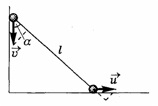
\includegraphics[width = 0.9 \textwidth]{0611EnergyAndImpulseBar.jpg}
\end{minipage}
\begin{ans}
$v_m = \frac{2}{3}\sqrt{\frac{2gl}{3}}$
\end{ans}
\end{ex}

\begin{ex}
(2002) Три одинаковых шарика массы $m$ каждый, скрепленные вдоль прямой двумя невесомыми стержнями длиной $l$, вертикально поставили на гладкую горизонтальную плоскость. Найти скорость верхнего шарика в момент удара о плоскость.
\begin{ans}
$v = \sqrt{24gl/5}$
\end{ans}
\end{ex}

\begin{ex}
(2018) Студент стреляет из рогатки шариком массой 20 г, доведя усилие при растяжении резинки до 50 H. При этом длина резинки увеличивается в три раза. Резника рогатки имеет общую длину в нерастянутом состоянии 30 см, сложена вдвое. 1) Определите скорость шарика пренебрегая массой резинки. 2) Определите скорость шарика, если масса резинки 50 г.
\begin{ans}
$v_1 = \sqrt{2FL/m}=27,4$ м/с, $v_2 = \sqrt{6FL/(3m+M)} = 20,2$ м/с
\end{ans}
\end{ex}

\begin{ex}
(2018) Автомобиль движется с постоянной скоростью по горизонтальному шоссе. Мощность, развиваемая двигателем
автомобиля, равна 60 кВт, эффективная площадь сопротивления автомобиля 0,7 м\textsuperscript{2} (площадка соударений молекул воздуха с автомобилем, перпендикулярная скорости автомобиля). КПД бензинового двигателя 25\%, удельная теплота сгорания бензина $46 \cdot 10^6$ Дж/кг, плотность бензина 710 кг/м\textsuperscript{3}. Температура окружающего воздуха $20^{\circ}$ С, атмосферное давление 10\textsuperscript{5} Пa, молярная масса воздуха 29 г/моль. 1) Сколько литров бензина тратит автомобиль за 1 час? 2) C какой скоростью движется автомобиль?
\begin{ans}
$Q = N/q \rho V = 26,5$ л/ч,  $v=\sqrt[3]{\frac{NRT}{2pS\mu}}=33$ м/с
\end{ans}
\end{ex}

\begin{ex}
\hspace{0pt} \\
\begin{minipage}{.65\textwidth}
(2016) Платформа массой $М$ стоит на гладкой горизонтальной плоскости. На платформе закреплен штатив, к которому на нити длиной $l$ подвешен груз массы $m$. Грузу сообщают горизонтальную скорость $v_0$, при этом максимальный угол отклонения нити от вертикали не превышает $90^{\circ}$. l) Определите максимальную высоту подъема груза. 2) Определите максимальную скорость платформы при качаниях груза. 3) Определите силу натяжения нити и момент времени, когда скорость платформы максимальна.
\end{minipage}
\begin{minipage}{.35\textwidth}
\centering
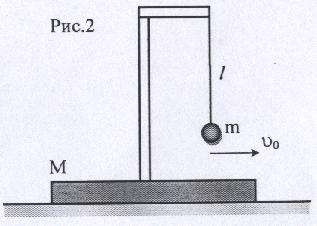
\includegraphics[width = 0.9 \textwidth]{PlatformWithOscillator.png}
\end{minipage}
\begin{ans}
$h= \frac{v_0^2 M}{2g(m+M)}$, $v_2 = 2mv_0/(m+M)$, $T=m(g+v_0^2/l)$
\end{ans}
\end{ex}
\section{Вращательное движение твердого тела}

\begin{wrapfigure}{r}{2.5cm}
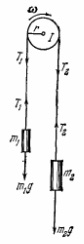
\includegraphics{0701RotationDynamicsAtwoodMachine.jpg}
\end{wrapfigure}

%1
\AddProb Определить ускорение тел и натяжение нити на машине Атвуда, предполагая, что $m_2>m_1$. 
Момент инерции блока относительно геометрический оси равен $I$, радиус блока $r$. Массу нити считать пренебрежимо малой. 

\AddProb Монета массы $m$ и радиуса $r$, вращаясь в горизонтальной плоскости вокруг своей геометрической оси с угловой скоростью $\omega$, 
вертикально падает на горизонтальный диск и прилипает к нему. В результате диск приходит во вращение вокруг своей оси. 
Возникающий при этом момент сил трения в оси диска постоянен и равен $M_0$. Через какое время вращение диска прекратится? 
Сколько оборотов сделает диск до полной остановки? Момент инерции диска относительно его геометрической оси~$I_0$. 
Расстояние между осями диска и монеты равно~$d$.

\AddProb Сплошной однородный короткий цилиндр радиуса $r$, вращающийся вокруг своей геометрической оси со скоростью $n$ об/с, 
ставят в вертикальном положении на горизонтальную поверхность. Сколько оборотов $N$ сделает цилиндр, прежде чем вращение его полностью прекратится? 
Коэффициент трения скольжения между основанием цилиндра и поверхностью, на которую он поставлен, не зависит от скорости вращения и равен~$\mu$.

\begin{wrapfigure}{r}{2cm}
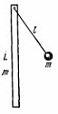
\includegraphics{0704RotationDynamicsBarAndBall.jpg}
\end{wrapfigure}

\AddProb Тонкий стержень массы $m$ и длины $L$ подвешен за один конец и может вращаться без трения вокруг горизонтальной оси. 
К той же оси подвешен на нити дины $l$ шарик такой же массы $m$. Шарик отклоняют на некоторый угол и отпускают. 
При какой длине нити шарик после удара о стержень остановится? Удар абсолютно упругий.

\AddProb (2015) Гимнаст массы 80 кг, крутя солнышко на турнике. остановился и сделал стойку на руках (вверх ногами). Затем. немного отклонившись. начал вращаться, удерживая тело a прямом положении. Оценить максимальную силу натяжения, возникающую в каждой руке гимнаста.

\AddProb Однородный тонкий негнущийся стержень массой $m$ поддерживается в горизонтальном положении двумя вертикальными опорами у концов стержня. 
В начальный момент времени $t$~ =~0 одна из опор выбивается. Найти силу, которая действует на вторую опору сразу же после этого момента.

\begin{figure}[h]
\centering
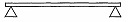
\includegraphics{0705RotationDynamicsHorisontalBar.jpg}
\end{figure}

\begin{wrapfigure}{r}{2.5cm}
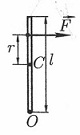
\includegraphics{0706RotationDynamicsSword.jpg}
\end{wrapfigure}

%6
\AddProb Каким участком сабли следует рубить лозу, чтобы рука не чувствовала удар? Саблю считать однородной пластиной.

\AddProb Шарик массой $m$ летит со скоростью $u_0$ навстречу покоящемуся стержню массой $M = 2m$ и длиной $2L$. 
Направление движения шарика перпендикулярно стержню и удалено на расстояние $l$ от его центра. 
После удара скорость шарика становится равной $u_1$, а стержня -- $V$. При этом стержень начинает вращаться с угловой скоростью $\omega$. 
Требуется определить 1) при каком $l$ шарик после удара остановится, а также 
2) скорость шарика, стержня и угловую скорость вращения стержня, если шарик ударяет в конец стержня.

\AddProb (2003 год) Обруч радиуса $R$ бросают вперед со скоростью $v_0$ и сообщают ему одновременно угловую скорость $\omega_0$. 
Определить минимальное значение угловой скорости, при котором обруч после движения с проскальзыванием покатится назад. 
Найти значение конечной скорости $v$, если $\omega_0 > \omega_{0min} $. Трением качения можно пренебречь.

\begin{wrapfigure}{r}{4cm}
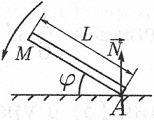
\includegraphics{0709RotationDynamicsFallOfBar.jpg}
\end{wrapfigure}

\AddProb Тонкий стержень массой $M$ и длиной $L$ свободно падает в вертикальной плоскости из начального положения, 
в котором угол между стержнем и горизонтальной плоскостью составлял $30^{\circ}$. 
Определите давление стержня на плоскость в момент удара, считая точку опоры стержня о плоскость неподвижной.

\AddProb Сплошной цилиндр без проскальзывания катится со скоростью $v$ по горизонтальной плоскости, 
которая переходит в наклонную поверхность с углом $\alpha$. Радиус цилиндра $R$. Какова должна быть $v$, чтобы цилиндр "не прыгнул"?

%11
\AddProb (2004) Двум дискам радиусами $R_1$ и $R_2$ сообщили одну и ту же угловую скорость $\omega_0$,
 а затем их привели в соприкосновение, и система через некоторое время пришла в новое установившееся состояние движения. 
Оси дисков неподвижны, трения в осях нет. Моменты инерции относительно их осей вращения равны $I_1$ и $I_2$. 
Найти приращение момента импульса системы и приращение ее механической энергии.

\AddProb Как надо ударить кием по бильярдному шару, чтобы при столкновении с другим (неподвижным) шаром 
1) оба шара стали двигаться вперед (удар с накатом), 2) первый шар остановился, а второй двигался вперед (удар с остановкой), 
3) второй шар двигался вперед, а первый откатился назад (удар с оттяжкой)? 
Предполагается, что удар наносится горизонтально в вертикальной плоскости, проходящей через центр шара и точку касания его с плоскостью бильярдного стола.

%Рассмотрим движение двух бильярдных шаров. Первым шаром назовем тот, по которому игрок ударяет кием, а вторым -- тот, 
%в который игрок старается попасть первым шаром. Как надо ударить кием, чтобы при столкновении первого шара со вторым: 
%1) оба шара стали двигаться вперед (удар с накатом), 2) первый шар остановился, а второй стал двигаться вперед (удар с остановкой), 
%3) второй шар двигался вперед, а первый откатился назад (удар с оттяжкой)? 
%Предполагается, что удар наносится горизонтально в вертикальной плоскости, проходящей через центр шара и точку касания его с плоскостью бильярдного стола.

\AddProb (2007) На гладком горизонтальном столе лежит однородный твердый стержень длины $l$ и массы $M$, 
в край которого ударяет твердый шарик массы $m$, движущийся со скоростью $v_0$, перпендикулярной к оси стержня. 
Считая удар идеально упругим и предполагая, что силы трения между поверхностью стола и лежащими на ней телами пренебрежимо малы, 
вычислить угловую скорость вращения стержня после удара.

\AddProb (2008) Сплошной однородный цилиндр, ось которого горизонтальна, движется без вращения по гладкой горизонтальной плоскости в направлении, 
перпендикулярном к его оси. В некоторый момент цилиндр достигает границы, где поверхность становится шероховатой и возникает постоянная 
(не зависящая от скорости) сила трения скольжения, а трение качения отсутствует. Каково будет движение цилиндра после перехода границы? 
Как распределится кинетическая энергия поступательного движения цилиндра?

\AddProb (2001) Пуля массы $m$, летящая горизонтально, попадает в покоящийся на шероховатой горизонтальной поверхности деревянный шар массой 
$M >> m$  и радиусом $R$ на расстоянии $l $ ниже центра масс и застревает в нем. Найти установившуюся скорость шара.

%16
\AddProb (2002) Шарик массой $m$ подвешен на нерастяжимой нити длиной $l$ и отклонен на малый угол от положения равновесия. 
В той же точке, что и нить, подвешен стержень длиной $1.5l$. Какова должна быть масса стержня $M$, чтобы в результате столкновения шарик остановился? 
Удар абсолютно упругий. Определить период колебаний шарика.

\begin{wrapfigure}{r}{4cm}
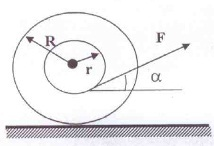
\includegraphics[width=4cm]{0717RotationDynamicsReelOfThread.jpg}
\end{wrapfigure}

\AddProb (2010) На горизонтальной шероховатой поверхности лежит катушка ниток массой $m$. 
Ее момент инерции относительно собственной оси $I$, внешний радиус $R$, радиус намотанного слоя ниток $r$. 
Катушку без скольжения начали тянуть с постоянной силой $F$, направленной под углом $\alpha$ к горизонту. Найти ускорение центра катушки.
%1. Дифуравнения в механике (трение, задачи о черепахах, лиса догоняет зайца, Туймадаа)
2. Распределенная масса, силы, канат
3. Вращательное движение (моменты инерции, сохранение момента импульса)
4. Колебания
5. Электростатика (сферы, потенциалы, конденсаторы)
6. ЭМ индукция, сила Ампера
7. Движение заряженных частиц в ЭМ поле
8. Переменный ток

%
%\chapter{Молекулярная физика}
%\section{Газовые законы}
%TODO Время удара футбольного мяча

\begin{wrapfigure}{r}{3cm}
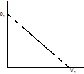
\includegraphics{082001GasLawsProcess.jpg}
\end{wrapfigure}

%1
\AddProb (2001) Какой максимальной температуры достигнет газ в процессе, изображенном на рисунке? Показатель адиабаты $\gamma$ считать известным.

\AddProb (2010) Посередине откаченной и запаянной с обоих концов горизонтально расположенной трубки длины $L$ находится столбик ртути длины $h$. 
Если трубку поставить вертикально, столбик ртути смеситься на расстояние $x$. Какое первоначальное давление в трубке? Плотность ртути $\rho$.

\AddProb (2013) В баллон, вместимостью $V$, при давлении $p$ нагнетают воздух. 
За какое время $t$ он будет накачан до давления $p_n$, если компрессор за время $\tau$ засасывает объем $V_0$ атмосферного воздуха? 
Температуру считать неизменной, а атмосферное давление равным $p_0$. Как изменится ответ, если воздух откачивать из баллона?

\begin{wrapfigure}{r}{3.5cm}
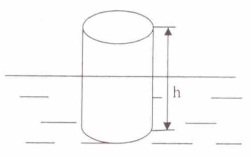
\includegraphics[scale=0.5]{082012GasLawsGlass.jpg}
\end{wrapfigure}

\AddProb (2012) На поверхности жидкости плотностью $\rho$ плавает тонкостенный цилиндрический стакан высотой $h$, наполовину погруженный в жидкость. 
На какую глубину $h_1$ погрузится стакан в жидкость, если его осторожно положить на поверхность жидкости вверх дном? 
На какую глубину $h_2$ нужно утопить перевернутый вверх дном стакан, чтобы он вместе с заключенным в нем воздухом пошел ко дну? Давление атмосферы $p_0$.

\begin{wrapfigure}{r}{2.5cm}
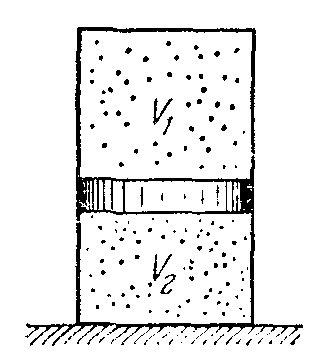
\includegraphics[scale=0.25]{0805GasLawsPiston.jpg}
\end{wrapfigure}

\AddProb В вертикальном закрытом сосуде имеется поршень, который может перемещаться без трения. 
По обе стороны от поршня находятся одинаковые массы одного и того же газа. 
При температуре $T$ объем верхней части в $n$ раз больше, чем объем нижней. 
Каким будет соотношение этих объемов, если повысить температуру до значения $T_2$?


\section{Молекулярно-кинетическая теория}

\begin{wrapfigure}{r}{5cm}
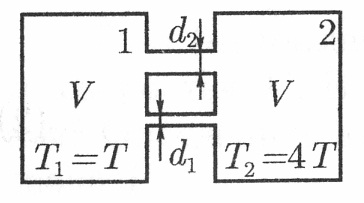
\includegraphics[scale=0.5]{0806KineticTheoryTwoVessels.jpg}
\end{wrapfigure}

%6
\AddProb Два сосуда одинакового объема соединены трубками. Диаметр одной из трубок велик, 
а другой мал по сравнению со средней длиной свободного пробега молекул газа, находящегося в сосуде. 
Первый сосуд поддерживается при температуре $T$, а второй при температуре $4T$. 
В каком направлении будет перетекать газ по узкой трубке, если перекрыть широкую трубку? 
Какая масса газа перейдет при этом из одного сосуд в другой, если общая масса газа в обоих сосудах равна $M$?

\begin{wrapfigure}{r}{3.2cm}
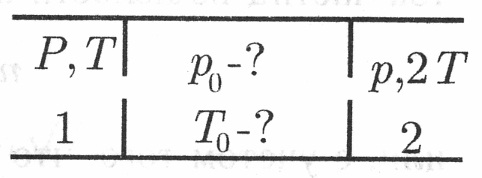
\includegraphics[scale=0.25]{0807KineticTheoryHelium.jpg}
\end{wrapfigure}

\AddProb Теплоизолированная полость небольшими малыми одинаковыми отверстиями соединена с двумя объемами, содержащими газообразный гелий. 
Давления в этих объемах поддерживаются одинаковыми и равными $P$, а температуры поддерживаются равными в одном из объемов $T$, в другом $2T$. 
Найдите установившиеся давление и температуру внутри полости.

\AddProb Плоская поверхность нагрета неравномерно, так что вдоль нее поддерживается градиент температуры $dT/dx$. 
В этих условиях газ, примыкающий к поверхности, приходит в движение вдоль поверхности. Это явление называют тепловым скольжением. 
Объясните его механизм и оцените скорость теплового скольжения. Необходимые параметры считать известными.

\AddProb (2008) Оценить по порядку величины установившуюся скорость, с которой будет двигаться в сильно разреженном воздухе плоский диск, 
одна из сторон которого нагрета до температуры $T_1$, а другая до температуры $T_2$, $T_1>T_2$. Температура воздуха равна $T$.

\AddProb (2009) Каково должно быть максимальное значение температурного градиента $dT/dz$ атмосферного воздуха, 
чтобы он мог находиться в устойчивом механическом равновесии? Воздух считать двухатомным газом с относительной молекулярной массой $\mu$. 
Ускорение свободного падения $g$ не зависит от высоты над поверхностью земли.
%\section{����� ���������� �������}

\begin{wrapfigure}{r}{2.5cm}
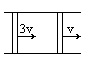
\includegraphics[scale=1]{0901LawOfConservationOfEnergyTwoPistons.jpg}
\end{wrapfigure}

%1
\AddProb � ������� ������������������ ������ ����� ����������� �������� ����� $m$ ��������� 1 ���� ������������ ���������� ���� ��� ����������� $T_0$. 
� ��������� ������ �������� ������� ���������� � ���� ������� � ����� $v$ � $3v$. �� ����� ������������ ����������� ��������� ���? 
������ ����� �� ��������, ������ ���� �� ��������� � ������ ������� ����������.

\AddProb (2004) � ������� �������������� ����� ����� ��������� ��� ������ ��� ������, ����� ������� $m$ � $2m$. 
����� ���� ��������� ��������� ���������� ������������ ���� ��� �������� $p$ � ������ $V$. 
� ���� ������ ������ ������� �������� � �������� �� ��������� $v_0$, ������� ������� ��������. 
������� ������������ �������� �������� ������.

\AddProb (2003) ������ ��������� ������������������� �������� � ��������� ����� ��������� �������������� ��������������� �������. 
��� ���������� ������� ����� ������� �� ��� ������ ����� � ����������� ���� ����� $T_0$. ������� ������ �������� ����������. 
����� ����������� ���� ��� ������� ��������� $\eta$ ������ ������� ����� � ������ ������� �����. ���������� �������� ����~$\gamma$.

\begin{wrapfigure}{r}{3cm}
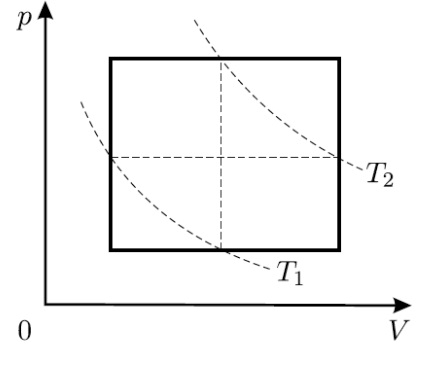
\includegraphics[scale=0.25]{0904LawOfConservationOfEnergyEfficiency.jpg}
\end{wrapfigure}

\AddProb ������� ��� �������� ������, ���� ������� ������� �� ���� ������ � ���� ������, � ������� ����� �������� ��������� ����������� ���. 
�������� ������ ������� � ����� ������� ����� �� ��������, ��������������� ����������� $T_1$, 
� �������� ������� ������� � ������ ������� -- �� ��������, ��������������� �����������~$T_2$.

\AddProb (2014) � ������������ �������������� ������ � ������������������� �������� ��� ������� ����� $m$~=~100~� ��������� 5 ���� ����� 
(�������� ����� 20 �/����). � ��������� ������ ������� ���������. ����� ����, ��� ������� ����������, ����� ���� ���������� � 2 ����. 
���������� �������� ����������� ����, ���� ��� ��������� ����������� ����� $T_0$ = 300~�. ��������, ��� ��� ������� ������. 
������� ����� ������� � �������� ������ �����������.

\begin{wrapfigure}{r}{3cm}
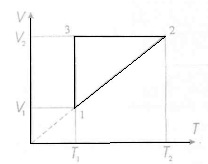
\includegraphics[width=3cm]{092002LawOfConservationOfEnergyProcess.jpg}
\end{wrapfigure}

%6
\AddProb (2002) ���� ����� ������ 1 ���� ���������� ���� � �������� ��������, ���������� �� �������? ����������� $T_1$ � $T_2$ ��������.

\section{������������}

\AddProb (1998) ������� ��������� ���, ������������ �������� ��� ���������� ������ ����� $C_V$. 
������� �������� ������������ ����� ���� ��� ������� ������, ���� �������� ���� �������� �� ������ $p=p_0~e^{\alpha V}$ ($p_0$ � $\alpha$ ��������).

\AddProb ������� ������������ ����������� ���������� ���� � ��������, ����������� �� ������ $P=P_0~-~\alpha~V^2$, 
��� $P_0$ � $\alpha$ -- ������������� ����������, $V$ -- ����� ������ ����.

\AddProb ��� ���������� ���� � �������� ����������� �������� $\gamma$ ������� ��������� �������� (� ����������� $V$, $T$), 
��� ������� ������������ ������� �� ����������� �� ������ $c=\xi~T^2$.

\begin{wrapfigure}{r}{4cm}
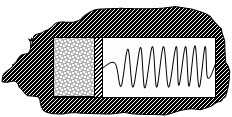
\includegraphics[scale=0.6]{092005HeatCapacityCylinder.jpg}
\end{wrapfigure}

\AddProb (2005) � ������������� ������������� �������� ����� �� ������������� ������ ��������� ���� ���� ���������� ����, 
� ������ ����� �������� - ������. ������� ��������������� �� ���������� �����, � �������, ������������� ����� ������� � �������, 
��������� ������������� � ����������������� ���������. ������� �����������, � ����� ������������ ���������� �����, ���������� �����, 
������������� � $\alpha$ ���. ��� ���������� ��� ���� ����������� � �������� ����? �������������� ��������, ������ � ������� ����������. 
����� ������������ ����.

\begin{wrapfigure}{r}{3cm}
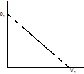
\includegraphics{082001GasLawsProcess.jpg}
\end{wrapfigure}

%11
\AddProb (2001) ��������� �������� ������������ $C_P(V)$ ���������� ����, ������������ �������, ���������� �� �������. 
���������� �������� $\gamma$ ������� ���������.
%
%\chapter{Электричество}
%\section{Электростатика}

%1
\AddProb Два маленьких шарика, массы которых $m$ и $M$, заряжены одинаковыми зарядами $q$ и удерживаются на расстоянии $L$ друг от друга. 
Шарики отпускают, и они начинают разлетаться. Найти скорости шариков после разлета на большое расстояние. 
Найти скорости шариков после разлета на расстояние $7L$.

\AddProb Точечный заряд $q$ находится между двумя заземленными проводящими концентрическими сферами 
радиусами $a$ и $b$ на расстоянии $r$ от центра ($a~<~r~<~b$). 
Найти полные индуцированные на сферах заряды. Рассмотреть все возможные предельные случаи.

\begin{wrapfigure}{r}{3cm}
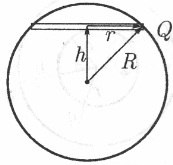
\includegraphics[width=3cm]{1003ElectrostaticsBall.jpg}
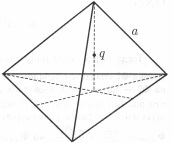
\includegraphics[width=3cm]{1004ElectrostaticsTetrahedron.jpg}
\end{wrapfigure}

\AddProb Заряженный металлический шар радиуса $R$ разрезан на две части по плоскости, отстоящей от центра на расстояние $h$. 
Найти силу, с которой отталкиваются эти части. Исходный заряд шара~$Q$.

\begin{figure}{h}
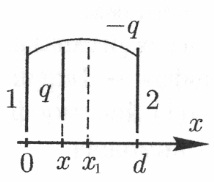
\includegraphics[scale=0.5]{1005ElectrostaticsTwoPlates.jpg}
\end{figure}

\AddProb Грани правильного тетраэдра со стороной $a$ равномерно заряжены с поверхностной плотностью заряда $\sigma$. 
В центр тетраэдра помещен точечный заряд $q$. Найти силу, с которой точечный заряд действует на одну из граней тетраэдра.

\AddProb Две большие проводящие пластины $1$ и $2$ расположены на расстоянии $d$ друг от друга, 
а между ними на расстоянии $х$ от пластины $1$ находится проводящая пластина с зарядом $q$. 
Крайние пластины соединены проводником и имеют заряд $-q$. 
Какой заряд пройдет по проводнику, соединяющему крайние пластины, если пластину с зарядом $q$ переместить из положения $x$ в положение с координатой~$x_1$.

\AddProb (2017) В вакууме относительно некоторой ИСО покоится однородное тонкое кольцо радиуса $R$, массой $3m$ и равномерно распределенным зарядом $q$. Какую минимальную скорость в этой ИСО должна иметь частица массой $m$ и зарядом равным по знаку и величине заряду кольца, чтобы, двигаясь вдоль оси кольца с очень большого расстояния, достичь его центра? Рассмотрите два случая: а) кольцо закреплено; б) кольцо свободное.

\section{Конденсаторы}

\begin{wrapfigure}{r}{4cm}
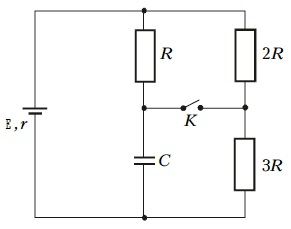
\includegraphics[scale=0.45]{1001Condensers.jpg}
\end{wrapfigure}

%6
\AddProb В электрической схеме, изображенной на рисунке, в начальный момент времени ключ $K$ разомкнут, конденсатор не заряжен. 
Параметры схемы указаны на рисунке. Определите начальные токи через резисторы и через батарею сразу после замыкания.

\begin{wrapfigure}{r}{3.5cm}
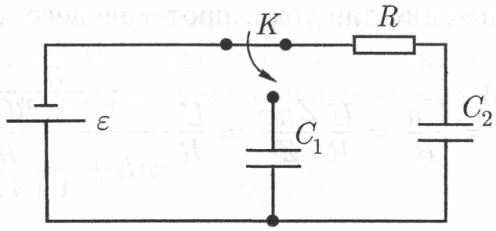
\includegraphics[scale=0.25]{1002Condensers.jpg}
\end{wrapfigure}

\AddProb Батарея с ЭДС, равной {\Large $\varepsilon$}, конденсаторы емкостями $C_1$ и $C_2$ и резистор сопротивлением $R$ соединены так, как показано на рисунке. 
Найдите количество теплоты $Q$, выделяющееся на резисторе после переключения ключа~$K$.

\AddProb По какому закону изменяется ток через конденсатор емкости $C$, подключенный к источнику тока $U$ через сопротивление~$R$?

\AddProb Две батареи включены в схему, изображенную на рисунке (сопротивления всех резисторов равны $R$). 
Первоначально конденсаторы не заряжены, а ключи разомкнуты. Ключи одновременно замыкают. 
1) Найти начальный ток через резистор $R_1$. 2) Какое количество теплоты выделится во всей схеме после замыкания ключей?

\begin{figure}
	\begin{subfigure}{0.5\textwidth}
	\centering
	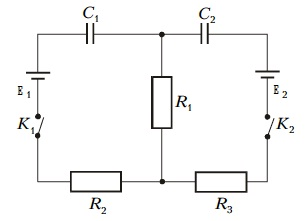
\includegraphics[scale=0.5]{1005Condensers.jpg}
	\end{subfigure}
	\begin{subfigure}{0.5\textwidth}
	\centering
	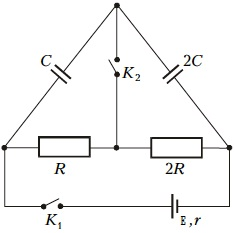
\includegraphics[scale=0.5]{1006Condensers.jpg}
	\end{subfigure}
\end{figure}

\AddProb В схеме на рисунке ключи разомкнуты, а конденсаторы не заряжены. Ключ $K_1$ замыкают, оставляя ключ $K_2$ разомкнутым. 
1) Какие напряжения установятся на конденсаторах? 2) Какой заряд протечет через ключ $K_2$ при замыкании?
%\section{���������� ������������� ���}

%1
\AddProb ����� ������������� ���� ����� ������� $�$ � $�$. ������������� ������� ��������� �������� � �����~$R$.

\begin{figure}[!h]
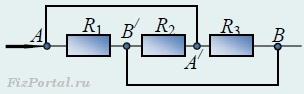
\includegraphics[scale=0.8]{1101DirectCurrentABCircuitLine.jpg}
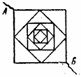
\includegraphics[scale=1]{1101DirectCurrentABCircuitStrange.jpg}
\end{figure}

\begin{figure}[!h]
\includegraphics[scale=0.5]{1101DirectCurrentABCircuitCube.jpg}
\includegraphics[scale=1]{1101DirectCurrentABCircuitStar.jpg}
\includegraphics[scale=0.5]{1101DirectCurrentABCircuitSquare.jpg}
\end{figure}

\AddProb ������������� ���������� $R_1$~=~1~��, $R_2$~=~2~��, $R_3$~=~3~��, $R_4$~=~4~��. 
���������� ��������� ���� $U$~=~1~�. ������� ���, ������� ����� ����� ���������.

\begin{figure}[!h]
\includegraphics[scale=0.4]{1102DirectCurrentFourResistors.jpg}
\end{figure}

\begin{wrapfigure}{r}{3.5cm}
\includegraphics[scale=1]{1103DirectCurrentThreeRings.jpg}
\end{wrapfigure}

\AddProb ��� ���������� ������ ������ ������� $r$ ��������� ���, ��� �������� �� �������. 
������� ������������� ���������� ����� ������� ������, ������� ���������� ������ � ������ $A$ � $B$. 
�������� ������������� ���� $\rho$, ������� ���������~$d$.

\AddProb ������� ������������� ������������� ����������� ������� (�� ���), ������� ������� �� ���������� ���������� �������������� $R$ ������.

\begin{figure}[!h]
\includegraphics[scale=0.5]{1104DirectCurrentFourInfiniteCircuit.jpg}

\includegraphics[scale=0.5]{1104DirectCurrentFourInfiniteCircuitAB.jpg}
\end{figure}

\begin{wrapfigure}{r}{2cm}
\includegraphics[scale=0.3]{1105DirectCurrentNet.jpg}
\end{wrapfigure}

\AddProb �� ����������� ���������� ���������� �����, ������ ����� ������� ����� ������������� $R$, ������� ���� ����� $AB$. 
������� ������������� ����� ����� ������� $A$ � $B$.

%6
\AddProb ������� $n$ �����, ������ �� ������� ��������� �� ����� ���������� �������� ����������� ������������ �������������� $R$. 
������� ������������� ����� ������ ����� ��������.

\AddProb ������������ ������ ����� ��� �������. ��� ��������� ����� �� ��� ������ �������� ����� 10 ���, ��� ��������� ������ -- ����� 15 ���. 
����� ����� ����� ������ �������, ���� ��� ��� ������� �������� ������ �����������, ���������������?

\begin{wrapfigure}{r}{4cm}
\includegraphics[scale=0.7]{1108DirectCurrentVDR.jpg}
\end{wrapfigure}

\AddProb �� ������� ����������� ������ ����������� ���� ���� �� ���������� �� ���������� ���������. 
���������� ���� ���� � ���� ��� ����������� ����� ��������� � ��������� ���� � ����������� 10 � � ���������� �������������� 100 ��.

\begin{wrapfigure}{r}{2.5cm}
\includegraphics[scale=0.45]{1109DirectCurrentArcDischarge.jpg}
\end{wrapfigure}

\AddProb �� ������� �������� ������ ����������� ���������� �� ��������� ���������� �������� ������� �� ����. 
���� ����������  � ��������� ����������� ���������� ��������������� � ����������. 
��� ����� ������������ �������� ������������� ��������� ���� ����� ������ ��� ���������� ��������� $U$~=~85~�?

\begin{wrapfigure}{r}{4cm}
\includegraphics[scale=1]{1110DirectCurrentResistorsAndGalvanometor.jpg}
\end{wrapfigure}

\AddProb �����, ������������ �� �������, ������� �� ���� ���������� ���������� $R_2$ � $R_3$ �������������� $R$ ������ 
� ���� ���������� ���������� ���������� $R_1$ � $R_4$, ������������� �������������� ������� ����� ��� $U~=~\alpha~I$. 
��� ����� ���������� ��������� ������� $U_0$ ���� ���� ����� ������������ ����� ����?
%\section{����� ���-������-�������}

%1
\AddProb ��� $I$ ����� �� �������� ������� ����������, ������� �������� ����� ����� ������� ���������� ������� $R$. ����� ��������� �������� �� ���~$O$.

\begin{wrapfigure}{r}{2.5cm}
\includegraphics[scale=0.4]{1202BiotSavartLawConductor.jpg}
\end{wrapfigure}

\AddProb ����� ������ � ����������� ����, ����������� �� ������� ����� ������� ���������� � ����� $I$ � ����� $O$, 
���� ��������� ������� ���, ��� �������� �� �������.


\section{���� ������}

\AddProb (2003) ������������� �������� ������ $m$ � ������ $L$ �������� �� ���� ������ �������� ������ $l$ � ��������� ���� � ��������� $B$, 
������ ������� ��������� �����������. � ������ ��������� �������� ��������� ����������� �������� $C$, ���������� �� ���������� $U$. 
������������� ������� � �������� ������������ ����. ����� ������������ ���� ���������� �������� �� ���������, 
���� �������� ������������ ���������� �� ����� ����� �����.

\begin{wrapfigure}{r}{4.5cm}
\includegraphics[scale=1]{122010AmperesForceLawTwoConductors.jpg}
\end{wrapfigure}

\AddProb (2010) ���������� ����� ����� ������ ������������� ������������ � ����� �� ���������� $a$ ���������� ���� ����� $m$, 
�������������� ����� �������������� �������� ������ ������ $l_1$ � ����������� � ������� ������� �������� ������ $l$. 
��������� ������������� ������ $\mu$. ������ �������� ���������� ��� ���� ���������. �� ���� ���� ����������� ����� ��� $J$. 
���������� ����������� ������� ��������� ��������� �����, ������, ��� � �������� ��������� ��������� �������� $T_0$ �� ����������. 
���������� ����������� ������������ �������� ���� ���� �� ��������� ��������, ������ ����������� ��������� ����� ��������, 
��� ������� ��������� � ������� ����������.


\section{������� � ���������� �������� ���������� ����}

\begin{wrapfigure}{r}{3cm}
\includegraphics[scale=0.25]{1205AmperesCircuitalLawDisc.jpg}
\end{wrapfigure}

\AddProb ���������� ��������������� ���� ������ $m$ ������� $R$, ���������� ���������� � ������ ������� $q$, 
������� � ���������� ��������� ���� � ��������� $B$. ����� ������� �������� ������� ����, ���� ��������� ��������� ����?

\begin{wrapfigure}{r}{4cm}
\includegraphics[scale=0.5]{1206AmperesCircuitalLawSphere.jpg}
\end{wrapfigure}

%6
\AddProb �� ����������� ������� ������������ ���������� ����� ������ $m$ ���������� ����������� ����� $q$. 
����� ����� �������� ��������� ������ ����� ������������ ���. � ��������� ������ ����� ���������, � ��������� ���� ���� ����� ����. 
�����, ��� �������� �� �������� ������� �������� ����� ��� ��������� ����������� ���������� ����, 
��������������� � ���� �������� ����� � ����������� �� ������� �� ��������� ������ $B(t)$.


\section{���������������� ��������}

\begin{wrapfigure}{r}{4cm}
\includegraphics[scale=0.5]{122002EMIFrame.jpg}
\end{wrapfigure}

\AddProb (2002) ������������� ����� �� ��������� $a$ � $b$ ��������� � ����� ��������� � ������ �����������, 
�� �������� ����� ��� $I$, �� ���������� $L$ �� ����. ����� ������� ������� ����� ��� ���������� ���� � �������, 
���� �������� ������������� ����� ����� $R$, � ���������� �������������� �� ����� ����������? 
�������, ��� �� ����� �������� �������� ����� ������� �� ������������.

\AddProb (2001) �� ���������� $a$ � $b$ �� �������� ������� ������� � ����� $I$ ����������� ��� ������������ ��� �������, 
��������� � ����� ������� �������������� $R$. �� �������� ��� ������ ������������ � ���������� ��������� $v$ ��������-���������. 
����������� �������������� ��������, ������� � ���������, ������� ����, ����������� ��� ����������� ����������� ��������. 
�� ����� ���������� �� �������� ������� ����� ��������� ����, ����� �������� �������� �������?

\begin{figure}[!h]
\includegraphics[scale=0.9]{122001EMIWiresAndBar.jpg}
\end{figure}

\AddProb (2004) ������������� �������� ����� $m$ � ����� $L$ �������� ������������� �� ���� ������ �������� ������ $h$ � ��������� ����, 
�������� �������� $B$ ���������� ����������� ����. � ������ ��������� �������� ��������� ����������� �������� $C$. 
�������� ������ �� ��������� ���������� � ���������. ���������� ������ ����� ��������� ������� $T$. �������������� ������� � �������� ����������.

\begin{wrapfigure}{r}{2cm}
\includegraphics[scale=0.5]{121998EMIConductorAC.jpg}
\end{wrapfigure}

\AddProb (1998) �� ���� ������������ ������, ����������� ����� �������������� $R$ � ������ ���������� � ��� {\Large $\varepsilon$} 
� ���������� �������������� $r$, ��� ������ �������� ��������� $AC$, ����� �������� $L$, ����� $m$. 
������� ��������� � ���������� ��������� ���� � ��������� $B$, ������������ �� �������. 
������� �������������� �������� ���������� � ���� ���� �������, ����������� ������� � �������������� ���� � ����������.

\begin{wrapfigure}{r}{4cm}
\includegraphics[scale=0.25]{1211EMIHillAndBridge.jpg}
\end{wrapfigure}

%11
\AddProb �� ���� ������������ ������������� ������������, ����������� ��� ����� $\alpha$ � ��������� � 
������������� �� ���������� $l$ ���� �� �����, ����� ��������� ��� ������ ������������� ��������� ������ $m$. 
������������ �������� ����� �� ������������ ����������� �������� $C$, � ��� ����������� ��������� � ��������� ����, 
�������� �������� $B$ ���������� �� ���������. � ��������� ������ ��������� ���������� �� ���������� $l$ �� ��������� "�����". 
���������� ����� $t$, �� ������� ��������� ��������� ��������� "�����" ����� ����, ��� �� ��������. 
��������� �������������� � �������������� ������� ����������.

\AddProb (2001) ��� ������������ ������ ���� ��������� � ��������� ��� �����  $\alpha$. 
�� ��� �������� ��� ��������� ���� ������� ������ ��������� ����� $m$. ���� �������� �������� � �������������� $L$. 
������� ��������� � ���������� ��������� ���� �������� $B$, ���������������� ���������, � ������� �������� ���������. 
����������� ������ ��������� � ���� ����� $\mu$. ����� ����� �������� �������� ���������? �������������� ���, ��������� � ������� ����������.

\begin{wrapfigure}{r}{4.5cm}
\includegraphics[scale=1]{122009EMICoin.jpg}
\end{wrapfigure}

\AddProb (2009) ������ ������ ������ $m$ �������� $R$ � �������� $d$ �������� � ���� ���� ������� � ���������� ��������� ���� $B$. 
������ �������� ���������� ���� ��������� ����� ��� ������ � ��������������� ��������� ���������� �������. ����� ��������� ������.

\begin{wrapfigure}{r}{5cm}
\includegraphics[scale=0.5]{1214EMIRailsAndBridge.jpg}
\end{wrapfigure}

\AddProb ������������ ������ ������ $2L$ ���������� �� �������������� ��������� �� ���������� $l$ ���� �� �����. 
� �� ������ ������������ ��� ���������� ������� � ��� {\Large $\varepsilon$}. �� ������� ����� ��������� ����� $m$, 
������� ����� ������������� ��������� ����� ���. ��� ������� �������� � ���������� ������������ ��������� ���� � ��������� $B$. 
������, ��� ������������� ��������� ����� $R$, � ������������� ������� ����� ������� �� ������� ����� $\rho$, ������� ������ ����� ���������, 
����������� ��� �������� ��������� �� ��������� ����������, ����������� ����������, ���������� �������������� ����������, 
�������������� ���������, � ����� �������������� ����.


\section{�������� ���������� ������}

\AddProb (2012) ��� ���������� ������� �������� � ���������� ��������� ���� $B$, ������ $q_1/m_1~ =~q_2/m_2$. 
�������� ��������� �������� ������ ���� � ��������� �������������� ��������.

%16
\AddProb (2013) ����� $q$ �������� � ���� ���������� �������� $B = \alpha~r/r^3$. 
������� �������� ��������, ��������� �� ������ ��������� ������� �������� ������.

\AddProb (2007) ���������� ������� �������� � ���������� ���������� ���������� ����� $E$ � $H$ � ����� 
� ����� �������� �������������� $F~=~-\gamma\,v$. ����� �������� ������� ����� ���� $E$, ����������� �� �������.

\AddProb (2008) ����������-������� ������ �������� � ���������� ��������� ����, ������������� $H$ �������� ��������������� ��������� ������. 
��������� ������� � ����������-������� ������ �� ����������� ����� � ������������ �������� $u$ ����� ��� ������ � 
������������ �������� $v_0$ ��������������� ���. ��� ����� ����� $L$ ������ ��� ��������� ������������ � ����� ����� ������?


\section{������������� ������}

\begin{wrapfigure}{r}{3.5cm}
\includegraphics[scale=0.5]{1219OscillatoryCircuitCCL.jpg}
\end{wrapfigure}

\AddProb ������� �� ���� ���������������� ����������� ������������� �������� $C$ ������ �������� �� ���������� $U$ 
� � ��������� ������ ������� ���������� � ������� �������������� $L$, ��� ��� ����������� ������������� ������. 
������ �������� ������� $\tau$ ���� �� ������������� �����������, � ������������� ����� ���������� ���������� ������ ����. 
������� ��������� ��������� ������ �� ���������� ������������.

\begin{wrapfigure}{r}{4cm}
\includegraphics[scale=0.4]{1220OscillatoryCircuitC1C2L.jpg}
\end{wrapfigure}

\AddProb ��� ������������ ���������� �������������� $C_1~=~C_2~=~C$ � ������� ������������� $L$ ��������� ���, ��� �������� �� �������. 
� ��������� ������ ������� ���� ���������, ����������� $C_1$ ������� �� �������� ����������� $U$, � ����������� $C_2$ �� �������, 
���� ���� � ������� ����� ����. ���������� ������������ �������� ���� ���� � ������� ����� ��������� ���� � ������ ���������������� ��������� � ����. 

\begin{wrapfigure}{r}{3.5cm}
\includegraphics[scale=0.5]{1221OscillatoryCircuitCLR.jpg}
\end{wrapfigure}

%21
\AddProb � �����, ������������ �� �������, � ��������� ������ ������� �������� ���� $K$, � ����������� �������� $C$, 
������� �������������� ����� $q_0$, �������� ���������� ����� ������� ������������� $L$. 
����� ��� ������� ��������� ������������� ��������, ���� $K$ ����� ���������. ����� ����� $Q$, ������� �������� ����� �������� $R$. 
������������� ����� � ������ ����������� ����� ������ $R$, � �������� - ���������� ������.

\begin{wrapfigure}{r}{3.5cm}
\includegraphics[scale=1]{122011OscillatoryCircuitTriangleCCCLLL.jpg}
\end{wrapfigure}

\AddProb (2011) ������������� ������ ������������ ����� �����������, ������ ������� �������� �������� ������� $C$, 
� ������� ��������� � ����� ����������� ������ ��������������� $L$. 
����������� �������������� � �������� ��������������, ������� ������� ��������� ���������.


\section{���������� ������������� ���}

\begin{wrapfigure}{r}{2cm}
\includegraphics[scale=0.4]{1223AlternatingCurrentCLR.jpg}
\end{wrapfigure}

\AddProb � ������������ �� ������� ������������� ���� ���������� ������� ������������ ����������� ����������, 
��� ������� ���������� ��� ����� ������������� �� ������� �� �������� $R$. ������������� $L$ � ������� $C$ ������� ����������.

\AddProb ��� ����� ������� ��������� ���� � ���� ������� ������ �� ��������� ������������ ����������, 
�� �� �� ��� �������? ������������� $L$, � ������� $C$, � ������������� $R$ ������� ����������.

\begin{figure}[!h]
\includegraphics[scale=0.5]{1224AlternatingCurrentCCLR.jpg}
\end{figure}

\AddProb � ����������� �� ������� ����� � ������ $t$~ =~0 �������� ���� $K$. ����� ����������� �� ������� ���� $I$, 
�������� ����� �������� �������������� ��� {\Large $\varepsilon$}~=~{\Large $\varepsilon_o$}\,$\sin\,\omega\,t$.
%$\varepsilon\,=\,\varepsilon_0\,\sin\,\omega\,t$.  
��������� ������� ������� ������������ $R\,=\,\sqrt{L/C}$.

\begin{figure}[!h]
\includegraphics[scale=0.5]{1225AlternatingCurrentCLRR.jpg}
\end{figure}
%
%\chapter{Колебания}
%\section{Колебания}

%1
\AddProb Груз массой $m$ прикреплен к пружине жесткостю $k$, а пружина к точке подвеса. 
Под действием внешней силы точка подвеса колеблется в вертикальном направлении по закону $x_p~=~A~\cos\,\omega t$. 
Какова амплитуда установившихся колебаний груза в вязкой среде, если сила сопротивления пропорциональна скорости $(F~=~-bv)$?

\begin{wrapfigure}{r}{2.2cm}
\includegraphics[scale=0.25]{1302OscillationsDynamicAbsorbentOfOscillations.jpg}
\end{wrapfigure}

\AddProb Схема динамического поглотителя колебаний представлена на рисунке. На первую массу действует гармоническая сила $F(t)~=~F_0\,\sin\,\omega\,t$. 
При каких условиях амплитуда вынужденных колебаний первой массы будет равна нулю?

\AddProb Найдите частоту колебаний точки с массой $m$, способной двигаться по прямой и прикрепленной к пружине, 
другой конец которой закреплен в точке $A$ на расстоянии $l$ от прямой. Пружина, имея длину $l$, натянута с силой $F$.

\AddProb Найдите частоту колебаний точки с массой $m$, способной двигаться по окружности радиуса $r$ и прикрепленной к пружине, другой конец которой закреплен в точке $A$, кратчайшее расстоянии то точки $A$ до окружности равно $l$. Пружина, имея длину $l$, натянута с силой $F$.

\begin{figure}[!h]
\includegraphics[scale=0.25]{1303OscillationsSpringAndLine.jpg}
\includegraphics[scale=0.25]{1304OscillationsSpringAndCircle.jpg}
\end{figure}

\AddProb Найти круговую частоту малых колебаний тонкого стержня массы $m$ и длины $l$ вокруг горизонтальной оси, проходящей через точку $O$. 
Жесткость пружины $k$. В положении равновесия стержень вертикален.

%6
\AddProb Молекулу одноатомного газа массы $m$, совершающую колебания около некоторого положения равновесия с амплитудой $a$ и частотой $\omega$, 
в первом приближении можно считать линейным гармоническим осциллятором. 
Найти $f(x)$ -- функцию распределения вероятностей значений координаты $x$ такого осциллятора, среднее значение координаты $\langle x \rangle$, 
среднее значение $\langle U \rangle$ потенциальной энергии осциллятора.

\AddProb Расположенный горизонтально цилиндрический сосуд объема $V$, заполненный $\nu$ молями идеального газа, 
разделен поршнем массы $m$, который может двигаться без трения. В равновесии поршень находится посередине цилиндра. 
При малых смещениях из положения равновесия поршень совершает колебания. Найдите зависимость частоты этих колебаний от температуры, 
считая процесс изотермическим. Площадь поперечного сечения трубки равна~$S$.

\begin{wrapfigure}{r}{3.5cm}
\includegraphics[scale=0.4]{1308OscillationsPistonInVerticalTube.jpg}
\end{wrapfigure}

\AddProb В длинной вертикальной цилиндрической трубке, закрытой с нижнего конца, может ходить без трения поршень, 
масса $M$ которого велика по сравнению с массой газа, заключенного внутри трубки. В положении равновесия расстояние между поршнем и дном трубки равно $L$. 
Определить период малых колебаний, которые возникнут при отклонении поршня от положения равновесия, в предположении, что они являются изотермическими, 
а газ идеальным. Площадь поперечного сечения трубки равна $S$, атмосферное давление равно $P_0$. Рассмотреть предельный случай, когда $P_0$~=~0.

\begin{wrapfigure}{r}{3cm}
\includegraphics[scale=0.5]{1309OscillationsDisc.jpg}
\end{wrapfigure}

\AddProb Тонкий однородный диск массы $m$ и радиуса $R$, подвешенный в горизонтальном положении к упругой нити, совершает крутильные колебания в жидкости. 
Момент упругих сил со стороны нити $M~=~\alpha\,\varphi$.  Сила сопротивления на единицу поверхности $F~=~\eta\,v$. Найти частоту малых колебаний.

\AddProb Идеальная жидкость объема $V$ налита в изогнутую трубку с площадью сечения канала $S$. Найти период малых колебаний жидкости.

\begin{figure}[!h]
\includegraphics[scale=0.5]{1310OscillationsPerfectLiquid.jpg}
\end{figure}

%11
\AddProb Трубка высотой $H$ наполнена жидкостью и соединена с наклонной трубкой (угол наклона $\alpha$). 
Каков будет период колебаний жидкости в такой системе?

\begin{wrapfigure}{r}{3cm}
\includegraphics{132006OscillationsRopeInTube.jpg}
\end{wrapfigure}

\AddProb (2006) В тонкой трубке может скользить без трения веревка длиной $L$. В начальный момент времени веревка находится в левом колене. 
Определить период колебаний $T$ веревки. Жесткостью веревки на изгиб пренебречь. 
Каким будет период колебаний $T_1$, если расстояние между вертикальными коленами трубки увеличить с $L$ до $2L$?

\AddProb (2004) На горизонтальной плоскости с коэффициентом трения $\mu$ лежит брусок массы $m$, который пружиной жесткости $k$ соединен с вертикальной стенкой. Брусок сместили на расстояние $9\mu mg /2k$ и отпустили. Найти число колебаний бруска до остановки.

\begin{wrapfigure}{r}{2cm}
\includegraphics[scale=0.25]{1314OscillationsPlanePendulum.jpg}
\end{wrapfigure}

\AddProb Найти период малых колебаний плоского маятника, точка подвеса которого с массой $M$ находится на гладкой горизонтальной прямой 
(масса маятника $m$ и его длина $L$).

\AddProb Дана проволочная вешалка, которая качается с малой амплитудой в плоскости рисунка относительно заданных положений равновесия. 
В положениях а и б длинная сторона вешалки расположена горизонтально. Две другие стороны равны между собой. 
Во всех трех случаях (а, б, в) возникают колебания с одинаковыми периодами. Где расположен центр масс вешалки?

\begin{figure}[!h]
\includegraphics[scale=0.35]{1315OscillationsHanger.jpg}
\end{figure}


\begin{wrapfigure}{r}{2cm}
\includegraphics[scale=0.25]{132007OscillationsTwoSpringsAndWeight.jpg}
\end{wrapfigure}

%16
\AddProb (2007) С какой частотой $\omega_0$ будет совершать малые вертикальные колебания в поле тяжести груз массы $m$, 
подвешенный на двух одинаковых пружинах жесткости $k$, образующих в равновесии углы $\beta$ с вертикалью?

\AddProb (2015)На гладкой горизонтальной поверхности находится грузик, прикрепленный двумя одинаковыми пружинами к стенкам (рис. 2, вид сверху). 
В положении равновесии грузика пружины имеют одинаковое растяжение~$\Delta l$. 1) В первом случае груз совершает малые колебания вдоль оси~$x$. 
Как зависит период этих колебаний от величины~$\Delta l$?   2) Во втором случае траектория грузика, совершающего малые колебания, изображена на рис. 3 
(в увеличенном виде). Определите $\Delta l$, если длина пружин в нерастянутом состоянии $l$~=~15 см. Во всех случаях выполняется закон Гука.

\begin{figure}[!h]
\includegraphics[scale=0.7]{132015OscillationsLissajousCurve.jpg}
\end{figure}

\begin{wrapfigure}{r}{4cm}
\includegraphics[scale=0.25]{132014OscillationsCondenserAndDoublet.jpg}
\end{wrapfigure}

\AddProb (2014) В центре плоского конденсатора удерживают диполь в положении 1, указанном на рисунке. 
Диполь представляет собой два маленьких заряженных шарика с зарядами $q$ и $-q$ и массами $m$ каждый, 
соединенных невесомым непроводящим стержнем длины $L$. Разность потенциалов между пластинами конденсатора равна $U$, 
расстояние между пластинами равно $d$ (много меньше размеров пластин). Диполь поворачивают вокруг его центра и переводят в положение 2, 
которое является устойчивым положением равновесия диполя. 
1) Определите работу электрического поля при повороте диполя из положения 1 в положение 2. 
2) Определите период малых крутильных колебаний диполя вокруг положения 2. 
3) Какую минимальную скорость нужно сообщить диполю в положении 2 параллельно пластинам для того, чтобы диполь улетел из конденсатора? 
Силу тяжести не учитывать.


\begin{wrapfigure}{r}{3cm}
\includegraphics{132013OscillationsMathematicalPendulum.jpg}
\end{wrapfigure}

\AddProb (2013) Точка подвеса математического маятника движется с постоянным ускорением $a$ (лежащим в плоскости колебаний маятника) 
в горизонтальном направлении. Найти закон движения маятника.

\AddProb (2010) На абсолютно гибкой нити подвешен маятник. Расстояния до точки подвеса равны $S_1$ и $S_2$. 
Статический прогиб в точке подвеса маятника равен $y_0$, а длина маятника $l$, его масса $m$. 
Принять, что при $t$~=~0 точка подвеса имеет вертикальное смещение $A$, а ее скорость $v_0$ равна нулю; маятник отклонен на угол $\varphi_0$. 
Считая, что натяжение нити $T = T_0 = const$, вывести дифференциальное уравнение малых колебаний маятника.

\begin{figure}[!h]
\includegraphics{132010OscillationsPendulumOnThread.jpg}
\end{figure}

\begin{wrapfigure}{r}{4cm}
\includegraphics[width = 4cm]{HittingRod.png}
\end{wrapfigure}
\AddProb (2017) Один конец однородного стержня длиной $L=1$ м закреплен на горизонтальной оси O (перпендикулярной плоскости чертежа), вокруг которой он может вращаться без трения. Другой конец стержня свободно лежит на опоре A, при этом стержень горизонтали. Свободный конец стержня приподнимают на
высоту $h = 1$ см относительно исходного положения, поворачивая стержень
вокруг оси O, и отпускают бы начальной скорости. 1) Определите скорость
свободного конца стержня при ударе об опору А. 2) Определите частоту ударов
стержня об опору А, считая удары абсолютно упругими и мгновенными.
Ускорение свободного падения $g$ = 10 м/с\textsuperscript{2}. Трением пренебречь.

\begin{wrapfigure}{r}{4cm}
\includegraphics[width = 4cm]{InvertedPenduumWithSpring.png}
\end{wrapfigure}
\AddProb (2016) Студент университета Пружинкин, увлекающийся физическим экспериментом (и не очень любящий теорию) смонтировал в физической лаборатории маятник. Маятник представлял собой очень легкий шарнирно закрепленный стержень длины $l = 50$ см (шарнир в нижней точке стержня), на котором были закреплены два одинаковых шарика c массами по $m = 0,9$ кг: один шарик -- в середине стержня, a другой нa верхнем его конце. Между стержнем и вертикальной неподвижной стенкой на высоте $h=3l/4$ от шарнира студент закрепил горизонтальные пружинки различной жесткости. В положении равновесия деформация пружинок была равна нулю. Для того, чтобы построить экспериментальный график зависимости периода малых колебаний от жесткости, студент изготовил для опытов пять пружинок с известными жесткостями $k = 10, 20, 30, 40, 50$ Н/м. Выведите выражение для периода колебаний маятника и предскажите результаты опытов Пружинкина.

\Closesolutionfile{solutions}
\Closesolutionfile{answers}

\chapter{Решения}
\Readsolutionfile{solutions}

\chapter{Ответы}
\Readsolutionfile{answers}

%\part{Чемпионаты по физике для студентов Физфака}
%
%\chapter{Студенческий чемпионат по физике 2006 года}
%\section{I ����}

\AddProb �� ������� �������������� ����������� ����� ��������� ����� ����� $m$ � ������� 
����� ����� $M$ ������ $H$. ����� ����������� �������� $v$ ���� ������� �����, ����� ��� 
������ ���������� ������?

\AddProb ������� ����� $M$ � ����� $L$ ������������ �����������, ��� ��� �� ������ ����� 
�������� �����. ���� ���������, � ��� ������ �� ����. ������ ����� ��������� �����, ����� 
����� ������� ����� $x$ ��� ����� �� ����?

\AddProb ������� �������������� ����� �������� ���� � ���������� ��������� $v_0$. � ������ $h$ 
��������� ��� ��������� �������� �����, ������� �������� ������������ �� �����. ������ 
����� ������ � ����� ��������, ����� ����������� �������� ������ �� ������� � ��������� 
�� ������.


\section{II ����}

\AddProb �� �������������� ��������� ����� ����� ����� �������~$V$. ������ �� 
����� ���������� ������ ������~$M$ ���, ��� ����� ������ ����������. ������� 
����������~$h$ ����� ������� � ����������, ���� ����������� �������������� 
��������� ����� $\sigma$ � ��� ����������� ��������� �� ����������� ������.

\AddProb ������� ����� $M$ � ����� $L$ ������������ �����������, ��� ��� �� ������ ����� 
�������� �����. ���� ���������, � ��� ������ �� ����. ������ ����� ��������� �����, ����� 
����� ������� ����� $x$ ��� ����� �� ����?

% ������ 1 ������� � ���������� ���������� ����(150)
\AddProb ���������� ��������������� ���� ������~$m$, �������~$R$, ������� � ���������� ��������� ���� ��������~$B$. 
����� ����� ���������� ����������� �� ��� ������ � �����~$q$. 
����� ������� �������� ������� ����, ���� ��������� ��������� ����?


\section{III ����}

% ����� ������ 1 ��� (152)
\AddProb ������������� ����� �� ��������� $a$ � $b$ ���������� �� ���������� $L$ �� 
������� ������� � ����� $I$. ����� ������� ������� ����� ��� ���������� ���� � 
�������, ���� �������� ������������� ����� ����� $R$, � �� ���������� 
�������������� ����� ����������?

% ������ 1 � ����� ���������� �������(115)
\AddProb � ������� ������������������ ������ ����� ����������� �������� 
����� $m$ ���������� 1~���� ������������ ���������� ���� ��� �����������~$T_0$. 
� ��������� ������ �������� ������� ���������� � ���� ������� � ����� $v$ � 
$3v$. �� ����� ������������ ����������� ��������� ���? ������ ����� �� 
��������, ������ ���� �� ��������� � ������ ������� ����������.

\AddProb ����������� ���� �������� �� ��� $\gamma$-������ � ��������� $E_1$\,=\,3100~��� � $E_2$\,=\,2000~���. 
����� ���� ������� ������� � ������������ ������� �������, ���� ������� ����� ����� $E_{\pi}$\,=\,135~���.
%
%\section*{Студенческий чемпионат по физике 2007 года}\addcontentsline{toc}{chapter}{Студенческий чемпионат по физике 2007 года}
%\section{I курс}

\AddProb К висящей очень лёгкой пружине жёсткостью $k$ подвешен шарик. Вначале пружина 
не растянута. Затем шарик отпускают. Какой максимальной скорости достигнет шарик 
при своем движении? Масса шарика $m$.

\AddProb Если смотреть на свет сквозь две гребёнки с разной частотой зубьев, наложенные 
друг на друга, то светлые участки будут чередоваться с тёмными. С какой скоростью 
будут перемещаться эти участки, если одну из гребёнок двигать относительно второй со 
скоростью 1 см/с? Неподвижная гребёнка имеет 5 зубьев и 5 промежутков между ними на 
сантиметр, а движущаяся~--~6.

% Задача (82) Энергия и импульс
\begin{wrapfigure}{r}{4cm}
\includegraphics[width=4cm]{0611EnergyAndImpulseBar.jpg}
\end{wrapfigure}

\AddProb Два тела малых размеров массой $m$ каждое соединены стержнем пренебрежимо малой массы длиной $l$. 
Система из начального положения у вертикальной гладкой стены приходит в движение. 
Нижнее тело скользит без трения по горизонтальной поверхности, верхнее - по вертикальной. 
Найдите значение скорости нижнего тела, при котором верхнее оторвется от вертикальной стенки.


\section{II курс}

\AddProb Если смотреть на свет сквозь две гребёнки с разной частотой зубьев, наложенные 
друг на друга, то светлые участки будут чередоваться с тёмными. С какой скоростью 
будут перемещаться эти участки, если одну из гребёнок двигать относительно второй со 
скоростью 1 см/с? Неподвижная гребёнка имеет 5 зубьев и 5 промежутков между ними на 
сантиметр, а движущаяся~--~6.

\AddProb Найдите частоту колебаний полярной молекулы в однородном электрическом поле, напряженность которого $E$\,=\,300~В/см. 
Полярную молекулу можно представить в виде жесткой гантельки длины $l\,=\,10^{-8}$~см, на концах которой находятся две материальные точки 
массы $m\,=\,10^{-24}$~г, несущие на себе заряды $e\,=\,1.6\times10^{-24}$~Кл и $-e$ соответственно. 

\AddProb Для определения отношения теплоёмкостей газа при постоянном давлении и при 
постоянном объёме иногда применяется следующий метод. Определённое количество газа, 
начальные объём и давление которого равны соответственно $V_0$ и $p_0$, нагревают 
платиновой проволокой, через которую в течение определённого времени проходит 
электрический ток: один раз при постоянном объёме $V_0$, причём газ достигает давления $p_1$, 
другой раз при постоянном давлении $p_0$, причём объём газа становится равным $V_1$. Как, 
измеряя эти величины, определить отношение теплоемкостей?


\section{III и IV курсы}

\AddProb Шар-зонд, имеющий нерастяжимую оболочку, поднялся на максимальную высоту и совершает малые колебания около равновесного уровня. 
Найдите период этих колебаний, считая, что на такой высоте плотность воздуха $\rho$ убывает с высотой равномерно на величину 
$\delta\,=\,1.2\times10^{-2}\,\rho$ через каждые $h$~=~100~м. Трением шара о воздух пренебречь.

\AddProb Однородно заряженный куб создаёт в своей вершине~$A$ электрическое поле напряжённостью~$E$. Из куба удалили кубик вдвое 
меньших размеров. Чему теперь будет равна напряжённость поля в точке~$A$?

\AddProb Оцените, за какое время застынет лед средней толщины $D$~=~0.5~м на озере во время холодной зимы. Считайте, что теплопроводность льда 
$\kappa$~=~2.2 Вт/(м$\cdot\,$К), удельная теплота кристаллизации $q\,=\,3.4\times10^5$ Дж/кг, плотность $\rho\,=\, 0.9\times10^3$ кг/м$^3$. 
Принять, что внешняя температура постоянна и равна $T_0\approx263$~К. 
%
%\chapter{Студенческий чемпионат по физике 2008 года}
%\section{I курс}

\AddProb Два тяжелых шарика брошены с одинаковыми начальными скоростями из одной точки вертикально вверх, один через $t$ секунд после другого. 
Они встретились в воздухе через $T$ секунд после вылета первого шарика. Определите начальную скорость шариков. Сопротивлением воздуха пренебречь.

\AddProb Подставка массы $m_1$ с полуцилиндрической выемкой радиуса $R$ стоит на гладком столе. 
Тело массы $m_2$ кладут на край выемки и отпускают. Найдите скорость тела и подставки в 
момент, когда тело проходит нижнюю точку полусферы. Трением пренебречь.

\AddProb Сплошной однородный короткий цилиндр радиуса $R$, вращающийся вокруг своей 
геометрической оси со скоростью $n$ об/с, ставят в вертикальном положении на 
горизонтальную поверхность. Сколько оборотов $N$ сделает цилиндр, прежде чем вращение его 
полностью прекратится? Коэффициент трения скольжения между основанием цилиндра и 
поверхностью, на которую он поставлен, не зависит от скорости вращения и равен~$\mu$.


\section{II курс}

\AddProb Однородный тонкий негнущийся стержень массой $m$ поддерживается в горизонтальном 
положении двумя вертикальными опорами у концов стержня. В начальный момент времени $t$~=~0 одна из  
опор выбивается. Найти силу, которая действует на вторую опору сразу же после этого момента. 

\AddProb Для определения отношения удельных теплоемкостей $c_P$ и $c_V$ газа измерили период $T_1$ малых 
колебаний ртути в U-образной стеклянной трубке с незапаянными концами. После этого на обе ветви 
трубки были насажены большие одинаковые полые стеклянные шары с исследуемым газом, вследствие 
чего период колебаний изменился и стал равным $T_2$. Считая процесс сжатия и разрежения газа в шарах 
адиабатическим, вывести формулу для $\gamma = \frac{c_P}{c_V}$. Объем каждого шара равен $V$ [см$^3$], давление газа в них в 
состоянии покоя $h$ [см рт. ст.], а площадь поперечного сечения трубки $S$ [см$^2$]. Объемом незаполненной 
части трубки можно пренебречь по сравнению с объемом шара~$V$.

\AddProb В плоский конденсатор размеров $L\times L\times d$ вдвигается с постоянной скоростью $v$ пластина 
диэлектрика с диэлектрической проницаемостью $\varepsilon$. Определить ток в цепи батареи с ЭДС $\xi$, 
подключенной к конденсатору.


\section{III курс}

\AddProb Материальная точка массой $m$, на которую не воздействуют внешние силы, 
невесомой нитью прикреплена к цилиндру радиусом $R$. Первоначально нить была 
намотана на цилиндр, так что материальная точка касалась цилиндра. В какой-то 
момент времени к массе $m$ приложен импульс силы в радиальном направлении так, что 
нить начала разматываться, начальная скорость массы $m$ составила $u$. Найти закон 
изменения длины смотанной нити.

\AddProb Идеальный одноатомный газ является рабочим веществом в цикле 1-2-3-1, изображенном на
рисунке. Участок 2-3 -- дуга окружности. Найдите КПД такого цикла.

\AddProb В плоский конденсатор размеров $L\times L\times d$ вдвигается с постоянной скоростью $v$ пластина 
диэлектрика с диэлектрической проницаемостью $\varepsilon$. Определить ток в цепи батареи с ЭДС $\xi$, 
подключенной к конденсатору.
%
%\chapter{Студенческий чемпионат по физике 2009 года}
%\section{I ����}

\AddProb ��� ���������� �������� � ����������� �� �������������� �������, ���������� 
������ ����. �������� ����������� $v_1$ � $v_2$. ���������� �� ����������� �� ����������� ��������� � �����~$L$. 
������ ����� ����������� ���������� ����� ������������ � �������� ��������?

\AddProb ����� ����� $M$ ��������� �� ���� ���������� �������, ����������� ��������� ���� �����. ���������� ����� ����� �������� ������� �����~$L$. 
����������� ������ ����� ������ � ������� �����~$\mu$. ������� ������ ��������� �����.

\AddProb ����� �������� $r$ �������� ������ � ���� ���� �������, �������� ������ ����������� ���, ������������� � �������������� ���������, 
� ������� ��������� $\omega$\,($\omega^2r > g$). ���������� ������ �������� ���������� ����� ������, ���������� � ������ ������ ��������� ���������, 
���� �������� ������� ������ �����~$v_0$.


\section{II ����}

\AddProb ���� ������ �� �������� � �����, ��������� ��� � �������, ����������� �� ���������� $h$ �� �����, �� ������� ����� ����. 
�� ������ ���� ������ ��������� ����, ����� ������� �������� ���� � ���������� �����, ���� ��� �������� �� ����� $v_1$, � �� ���� $v_2$ ($v_1>v_2$).

\AddProb ������������� ����� ����������� ����������� � ���������� ��������� ����, ������ �������� $\vec B$ �������� ��������� ��������������� ��������� �����. 
����������� ���� �� ��������� ����� �������� �������� ������������� �������� $AC$. �������� ��������� � ������������� �������� � 
������������� ��������� �����, �� �������� ��� ������. ���������� �������� �������� ������� ����� ����� $t$ ����� ������ ��������. 
����� ������� $m$, ������������� ������������� $R$, ���������� ����� ���������� $L$. ������������� �������������� � �������������� ����� ����������.

\AddProb ��������� ���� �������� �� �������� �����������, ������� �������������� ����� (��������� ����������� $y = ax^2$, ��� $a$ -- ���������). 
����������� ������ ����� ����� � ������������ $\mu\ll 1$. � ��������� ������ ������� ���������� ���� $x_0 = 2.75\mu/a$, � �������� �������. 
������ ����� ���������� ����, ����� ��� ������������ �����������?


\section{III ����}

\AddProb ������ ������� ����� ������� $R$ ��������� ��������� ����� ����� $m$ � ������� $+q$. ����� ����� $Q$ ����� ��������� � ������ ����� �����, 
����� ����� ����������� � ������� �����? ������������ ����� ����� ����������.

\AddProb ����� ����� ������������ �������� ������ ������� $R_0$, ������������ � ���������� ����������, ������� ����� ����� $L$ � ������ ������ $r$. 
������������� ��������� $\sigma$, �������� �������~$\eta$.

\AddProb ������� � ������� $q$ � ������ $m$ �������� � ��������� ��������� $v_0$ � ������ ����� � ���������� ��������� ���� � ��������� $\vec B$. 
���� ������� ������ ����� $\vec F = -r\vec v$, ��� $r$ -- ���������. �� ����� ���������� �� ��������� ����� ������� �����������?
%
%\chapter{Студенческий чемпионат по физике 2010 года}
%\section{I ����}

\AddProb � U-�������� ������ �������� ������� ������������ ����. �������� ��������� � ������ ����� ����� $v$, ���������� �- $u$. 
� ����� �������� �������� ������?

\AddProb ������ ����� $m$ ����� �� ���� ���, ��� �� �������� � ���������� ��������� �� �������������� ��������� � ������������� ������ $\mu$. 
����� ���� $\alpha$, ��� ������� ��������� ���� ����������. ���� ��� �����?

\AddProb ���������� ��� ������� $r$ ����������� ��� ���������� � ������� ����� ������� $R$. ����� ������� �������� ���� ����� ������ �� �����. 
��������� �������� ���� ������������ ����.


\section{II ����}

\AddProb �� ������� ����� ����� ������ ������ ����� $M_1$ � ������� $R$. �� ���� ������ ������ ����������� ������ ������ �� �������, 
������� ��������� � ������� ��������� $\omega$. ����� �������� ������ $M_2$. ����������� ������� ������� ������ � ����, ����������, 
����� ������� �������� �������� ����� �� ����� ����������� ����� ������� ���������� �������. ������� ����� ��������� ��� ������������ ��������?

\AddProb ������ ������ �������� � ���� ����� ��������� ����������. � ���� ������ �������� ������� ������������ ����. 
�������� ������� ����, ��������� � �����, ����� $v$, �������� ����� ����� $2v$. ��� �������� ��������� ����������. 
����� ������� ���� � ����� �������� � ������������ ���������? ���� ����� ��� ��������?

\AddProb ������������� �������� ������ $m$ � ������ $l$ �������� �� ���� ������ �������� ������ $R$ � ��������� ���� � ��������� $B$, 
������ ������� ��������� �����������. � ������ ��������� �������� ��������� ����������� �������� $C$, ���������� �� ���������� $U$. 
������������� ������� � �������� ������������ ����. ����� ������������ ���� ���������� �������� �� ���������, 
���� �������� ������������ ���������� �� ����� ����� �����.


\section{III ����}

\AddProb ������ ������ �������� � ���� ����� ��������� ����������. � ���� ������ �������� ������� ������������ ����. 
�������� ������� ����, ��������� � �����, ����� $v$, �������� ����� ����� $2v$. ��� �������� ��������� ����������. 
����� ������� ���� � ����� �������� � ������������ ���������? ���� ����� ��� ��������?

\AddProb �� ���� ������������ ������, ����������� ������ � ����� ��������������� $R$, ����� ��������� ��� ������ ���������, 
����� �������� $L$, ����� $m$, ������������� $R$. ������� ��������� � ���������� ��������� ����, �������� �������� $B$ ��������������� ��������� �������. 
����� ������������ �������� ���������� � ���� ���� �������, ���� ���������� �������������� ����.

\AddProb ������������������ �������������� ����� �������� ���������������� ������� �� ��� ������ ����� ������� $V$ ������. 
�������� ������������ ���� � ����� �������� ������ $p$, � ������ $2p$, � ����������� ���� � �� �� � ����� $T$. ������� ������������ ����� ����. 
���������� �������� �������� � ����� ������ ������ ����� ���������� ���������� ���������, ���� ������� ������������ ������ ������ ��� ������.
%
%\chapter{Студенческий чемпионат по физике 2011 года}
%\section{I ����}

\AddProb ��� ���� ������� ������������ �� ����� �����: ���� ����������� �����, ������ ��� ����� $\varphi~=~30^{\circ}$ � ���������. 
��������� �������� ������� ���� $v$~=~10 �/�. ����� ���������� ����� ������ ����� $t$~=~1~�.

\AddProb ������ �������� ����� $m$ � ����� $l$ ����� �� ������� �������������� �����������. ������������� ����� ����� $m$ �� ��������� $v$, 
���������������� � �������, ��������� �� ���� �� ��� ������ � ��������� � ����. ����� ���������� ������� ��������� ��� ����� �����?

\begin{wrapfigure}{r}{3cm}
\includegraphics[scale=0.5]{1309OscillationsDisc.jpg}
\end{wrapfigure}

% ����� ������ (179) ���������
\AddProb ������ ���������� ���� ����� $m$ � ������� $R$, ����������� � �������������� ��������� � ������� ����, ��������� ���������� ��������� � ��������. 
������ ������� ��� �� ������� ���� $M~=~\alpha\,\varphi$.  ���� ������������� �� ������� ����������� $F~=~\beta\,v$, ��� $v$ -- ��������� �������� 
�������� �����. ����� ������� ����� ���������.


\section{II � III �����}

\AddProb ��������� ����� � ������� ������������� ����� �������������� � ���������� ��������� $v$. ������� ����� ����� $h$. 
����� ������� �������� ������� ��� ������� ������� $t$, ���� � ������ ������� $t$~=~0 ������ �������� ���� ��������� ����� ����� $R$.

\AddProb � ����� ����� ����� �� ����� �����, ����� ���, �������� � ������, ����������� ����������� ����� � ���������� ��������� $v$? 
����� ���� $m$, �� ����� $l$.

\AddProb ������� ������� �� �������� �������� �������� $r$ � ���� ������� ��������� ��������� $R > r$. ������� ������ ������ ������ ���������� �� ������� 
��������� �������: ������� ���������� ���� �� ������� ���������, � ����� ���������� ���������� ���� �� ������ �� ������� ������� � ��� �� 
�����������, � ����� �������� �������. ����� ���������� ������� ������� ������ �� �������������� ����, ���������� � ���������� ���������� ��������� ���� $B$, 
����� �������� �������� ����������� ��� �������. � ������� ����� �������, �������� �� �����, ������������ ��������� ���������, � ������ ����� �������, 
���������� ������������ ����������� ��������, ������������ � �����������, �������� ������ ����� ����������� ����� � ���������� ��������� $v$ � �����������, 
���������������� ��� �������. ������, ��� ������� ������� �� ����� ��� ���������������, ������� ��������� ����������.
%
%\chapter{Студенческий чемпионат по физике 2012 года}
%\section{I ����}

\AddProb ���������� �������� ������ $m$ � ������ $L$ ������� � �������������� ��������� � ������� ��������� $\omega$ ������ ������ �� ��� ������. 
������� ����������� ��������� ������� �� ���������� $x$ �� ��� ��������, ���� �� ������ ����� ��������� ��������� ������ ������ $M$.

\AddProb ������� ��������� ������� �� ���� ���������� �������  ����������� $V_0$ ������, ����������� ������� ����� $L$ � ������� $S$. 
������ ����������� ����� �����. ������ ��������� �����. ���� ����������� ���� � ����� ������� ���������, ����� ��������� ���������� ������. 
���� ����� ������� � ��������� � ������������ $T_0$. �������������� ���������, ������ ����������� ����������� ���� �� ������ ������ 
�� �������� ����� �� ��������� ����������.

\AddProb ���������� ������� ������� $R$ � ����� $m$ �������� � ��������� ��������� $v_0$ ��� �������� ����� �������������� ���������. 
����� ����� ����� ����������� ���������������, ���� ����������� ������ �������� � ��������� ����� $\mu$? ����� ����� ��������� ������� �������� � �����?


\section{II � III �����}

\AddProb ������� ��������� ������� �� ���� ���������� �������  ����������� $V_0$ ������, ����������� ������� ����� $L$ � ������� $S$. 
������ ����������� ����� �����. ������ ��������� �����. ���� ����������� ���� � ����� ������� ���������, ����� ��������� ���������� ������. 
���� ����� ������� � ��������� � ������������ $T_0$. �������������� ���������, ����� ����������� ����������� ���� �� ������ ������ 
�� �������� ����� �� ��������� ����������.

% ����� ������ (185) ���������
\AddProb ����������� ������� �������� � ����� ���������� � ��������� ������� ������������ �������� ��������� ����������. 
� ���������� � � � ������� ������� ������� ����������� �������������. ��� ������ ������� ����� ����� �����. 
�� ���� ���� ������� (�, �, �) ��������� ��������� � ����������� ���������. ��� ���������� ����� ���� �������, ���� ������������� ����� � ������� ����������?

\begin{figure}[!h]
\includegraphics[scale=0.35]{1315OscillationsHanger.jpg}
\end{figure}

\AddProb ����� ����������� ���������� ���������� �������� � ���������� ������������� ���������� $\sigma$. 
� ������ ���������� ������� �������� ����� $ $. ���������� ����, � ������� �������� ����� ��������� �� ���� �����. �������������� ������ �� ���������. 
%
%\chapter{Студенческий чемпионат по физике 2013 года}
%\section{I ����}

\AddProb �������� ������� ������ ������ ����� $l$ ������������ �� �������. ����� �� ��� ����� � ��������� �������, ����� ����� ��������� � ���������� $a$. 
�������� ����� �� ������� �� ��������� $v$. ����� ����� ����� �� ������� �����?

\AddProb ������� ����� $m$ ������� � �������, ��� �� ��� ��������� ���������� ����, ���������������� ���������� ����� �������� � �������� �������. 
������� ��� �����������, ���� ������� ������������� ������� � ������� ���������� ��������������� �� ���������� ��������: $l~=~\alpha\,p$.

\AddProb ��������� ����� $A$ �������� �� ��������� ���������, ������������ ���� $\alpha$ � ����������, � �������� ��������� �������� $v_0$. 
����� ����������� �������� ����� �� ���� $\varphi$, ���� ����������� ������ $k~=~ \tg \alpha$ � � ��������� ������ $\varphi_0~=~\pi/2$.


\section{II ����}

\AddProb �������� ������� ������ ������ ����� $l$ ������������ �� �������. ����� �� ��� ����� � ��������� �������, ����� ����� ��������� � ���������� $a$. 
�������� ����� �� ������� �� ��������� $v$. ����� ����� ����� �� ������� �����?

\AddProb ��� ���������� ������, ������� ���������� ������ $q$, ��������� ��������. ������ ���������� ���, 
��� ���������� ����� ���� �������� �� $l$ �� $4l$. ����� ��������� �������, ���� �� ����� � ��������� ��������� �����~$2l$.

\AddProb ��������� ���������� ������ � �������, ����������� � �������� ������ ����� � ������, � ������� ����� ����� �������� ������� �������. 
��� ������� � ������ ��������� �� ���������� $R$ �� ��� ��������� �������. ����������, � ����� ������� ��������� ����� ������� ������� ������ ���� ���, 
����� �������� ������� ���������� � $n$ ���. ��������� �������� ������� $p_0$, ��������� ����� $\rho$, �� ������� � ������ ����� ������� ����������.
%
%\chapter{Студенческий чемпионат по физике 2014 года}
%\section{I курс}

\AddProb Под каким углом к горизонту следует бросить камень с вершины горы с уклоном $ 45^{\circ}$, 
чтобы он упал на склон на максимальном расстоянии от точки броска?

\AddProb На внутренней поверхности конической воронки с углом $2\alpha$ при вершине на высоте $h$ от вершины находится малое тело. 
Коэффициент трения между телом и поверхностью воронки равен $\mu$. 
Найти минимальную угловую скорость вращения конуса вокруг вертикальной оси $\omega$, при которой тело будет неподвижно в воронке.

\AddProb Моль одноатомного идеального газа нагревают в цилиндре под поршнем, удерживаемым в положении равновесия пружиной, подчиняющейся закону Гука. 
Стенки цилиндра и поршень адиабатические, а дно проводит тепло. Начальный объем газа $V_0$, при котором пружина не деформирована, подобран так, 
что $p_0\,S^2\,=\,k\,V_0$, где $p_0$ -- наружное атмосферное давление, $S$ -- площадь поршня, $k$ -- коэффициент упругости пружины. 
Найти теплоемкость газа для этого процесса.


\section{II и III курсы}

\AddProb Под каким углом к горизонту следует бросить камень с вершины горы с уклоном $ 45^{\circ}$, 
чтобы он упал на склон на максимальном расстоянии от точки броска?

\AddProb Два однородных тонких стержня одинаковой длины и разной массы $m_1$ и $m_2$ лежат на гладкой поверхности параллельно друг другу. 
Стержни могут вращаться без трения вокруг вертикальных неподвижных осей, отстоящих друг от друга на удвоенную длину стержней. 
Свободные концы стержней соединены невесомой пружиной жесткости $k$. Найти период малых колебаний системы.

\AddProb На рисунке изображена схема электромагнитного насоса для перекачки расплавленного металла. 
Участок трубы с расплавленным металлом помещается в магнитное поле, перпендикулярное оси трубы; 
через этот же участок в перпендикулярном (к магнитному полю и оси трубы) направлении пропускается ток. 
Найти избыточное давление $\Delta P$, создаваемое насосом. Величины, обозначенные на рисунке, считать известными.
%
%\chapter{Студенческий чемпионат по физике 2015 года}
%\section{I ����}

\AddProb ���� ������ �� �������������� ������ � ���������� ��������� $u$. 
� �� ������ ������ ��������� �������, ������ ������ ��� ������ ��� ����������, 
�. �. � ������ ������ �������� ����� $v$ ���� ���������� ����� �� ���� ��� ����� $\alpha$ � ���������. 
�� ����� ������ ������ ����, ���� ������ �� �� ����� � ��?

\AddProb ������� ����� �������� $R$ ��������, ��������� � �����, �������� �� ���� � ������� ����������� �����, ���������� �� ����� $l$. 
��� ����� ��������� ������������ ������ ����� �������� � ������ ��� ��������?

\AddProb �������� ������ � ��������� ����� � �������� �������� �������� ��������� ��������� ����, 
��������� �� ������� 1--2, �������� 2--3 � �������� 3--1. 
����� ��� ������ ��� ������� ������������ $T_2$ � ����������� $T_1$ ����������, ����������� ����� � ���� �����.


\section{II � III �����}

\AddProb ������������ ����� ������ $m$ �������� ��������� �� �������� $v_0$ � ������ �����, � ������� �� ���� ��������� ���� ����������������� �������������, 
���������������� �������� ��������: $F~=~-\beta\,v^2$, ��� $\beta$ -- ���������� ����������� �������������, ��������� �� ����� ����. 
���� ��������������� ���������� �� ���� �� ���������. ������� ����������� ����������� ���� �� �������. 
����� �� ���� ������������, ���� ��������� ��� �������� � ������ ������ ������?

\AddProb ���������� �������������� ���� ����� $M$ � ������� $R$ ����� �������� �������������� ������ �������������� ��� $O$. 
�� ���� ������ �������� ����, � �������������� ����� ������� ���������� ���� $A$. 
���� ���� �������������� �������� ���� ����� $m$, ����������� �� ����� �����, ��� ������������ �������� ���� $\alpha$. ����� ������� ����� ��������� �������.

\AddProb ��� ����� ������� ��������� ���� $I$ � ����, ������������ �� �������, ������� ������ �� ��������� ������������ ���������� 
$U~=~U_0\,\cos\,\omega\,t$, �� �� �� ��� �������? ����� ��� ���� ������� �������� ��� ����� ����������� ����������� � ����������� �� ������ $RC$-����.
%
%\part{Олимпиада "Юные таланты"}
%
%\chapter{Олимпиада "Юные таланты" 2008 года}
%\section{10 �����}

\AddProb ����� ������������� ���� ����� ������� $A$ � $B$. ������������� ������� ��������� �������� � �����~$R$.

\AddProb ������ ������� �������� � ������� ����� $m$ �� ����� �������� ��������� � ������������ ��������� ������ �����~$O$. 
��������, ��� � ������� ����� ���������� ������ ���� ��������� ������� ����� $T$ � � ��� ���� ������, ��� � ������. 
������� ��������� ��������� ������ � ������� � ������ ������ ����������. ��������� ���������� ������� �����~$g$.

\AddProb � �������, ������������ �� ������ 20 �, ������� ��� �� ��������� 20~�/�. 
��� ������ ��������� � ����� ��������� ���� � ������ �� ����� ��� ��������. ���������� ���������� �� ��������� ����, ���� ����� ������ ���� 1,4~�.

\AddProb � �������������� ������� � ����� ������� ������ ������ $L$ � �������~$S_1$. 
��� ������ ������ ����� ������ �������� �������� �� ��� �������. ����� ������ ��� ���� ���������? 
������� ������� $S_2\,=\,2S_1$, ��������� ������ ���� � ������� ���� $L$, ��������� ��������� ������ $\rho\,=\,0.5\rho_B$, , ��� $\rho_B$ -- 
��������� ��������� ����.



\section{11 �����}

\AddProb � ����� ����������� ������� ������� ����� $l$ ���������� ����, � ���������� ���� �� ����� �������� ��~$2l$. 
�����������, ��� ��������� ������� ��������������� ��������, ����� ������� �������� �����, 
������������ �� ���� ������� �� ����� � �������������� ���������, ���� ����� ������� � ���� ������~$L$. ������ ������� ����������.

\AddProb �� �������������� ����������� ����� ��� ���������� ������ ������~$M$. 
����� �������� �������� ������� ���� ������ $m$ � ����� ��� �������~$2\alpha$. ���� ����� ��������� �������? ������� ����������.

\AddProb � ������� ����������� ���������� � ���������� ��������� $v$ �������� �� �����������. 
���������� ��� � ���� �������, ������������ � ������������. ������� ��������� ��� ������� $E$, ��������������� ������������� {\Large $\varepsilon$}, 
������ �������� $h$, ������� ���������� ������� ������������~$S\,=\,b^2$.

\AddProb 4.	����������� ��� ��������� � ��������� ��������. ��������, ��� ��� ���������� ������� ��������������� �������� ������. 
������� ������, ������� ��������� ��� ��� ��������� ��� ���������� �������~$Q$.

%
%\chapter{Олимпиада "Юные таланты" 2009 года}
%\section{10 класс}

\AddProb Радиус рукоятки колодезного ворота в $3$ раза больше радиуса вала, на который наматывается трос. 
Какова линейная скорость конца рукоятки, если ведро с глубины $10$~м поднимается за $20$~с.

\AddProb Оцените, до какой температуры нужно нагреть воздух внутри оболочки воздушного шара объемом 500 м$^3$, 
чтобы он мог поднять человека массой 70~кг? Масса оболочки шара равна 30~кг.

\AddProb Гиря массой $m$ падает на чашку пружинных весов с высоты $H$ и испытывает абсолютно упругий удар. 
На какую величину $h$ сожмется пружина весов после удара, если масса чашки равна $M$, а коэффициент жесткости пружины равен $k$?

%Задача 118, молекулярка, ЗСЭ
\begin{wrapfigure}{r}{3cm}
\includegraphics[scale=0.25]{0904LawOfConservationOfEnergyEfficiency.jpg}
\end{wrapfigure}

\AddProb Найдите КПД тепловой машины, цикл которой состоит из двух изохор и двух изобар, а рабочим телом является идеальный одноатомный газ. 
Середины нижней изобары и левой изохоры лежат на изотерме, соответствующей температуре $T_1$, 
а середины верхней изобары и правой изохоры -- на изотерме, соответствующей температуре $T_2$.



\section{11 класс}

\AddProb По первоначальным предположениям Бора, электрон в водородном атоме движется по круговой орбите. 
С какой скоростью $v$ должен двигаться такой электрон, если заряд электрона $q_1\,=\,-1.6\cdot~10^{-19}$~Кл, 
заряд ядра $q_2\,=\,1.6\cdot~10^{-19}$~Кл, радиус орбиты можно принять равным $r\,=\,0.5\cdot 10^{-10}$~м, масса электрона $m\,=\,9.1\cdot 10^{-31}$~кг.

\AddProb Ящик, имеющий форму куба с длинной ребра $L$, находится на горизонтальной поверхности. 
При каких значениях коэффициента трения между ящиком и поверхностью работа при перемещении ящика волоком на расстояние $L$ будет больше, 
чем работа при кантовании (опрокидывании через ребро)?

% Задача 159, электричество, ЭМИ
\begin{wrapfigure}{r}{5cm}
\includegraphics[scale=0.5]{1214EMIRailsAndBridge.jpg}
\end{wrapfigure}

\AddProb Параллельные рельсы длиной $2L$ закреплены на горизонтальной плоскости на расстоянии $l$ друг от друга. 
К их концам подсоединены две одинаковые батареи с ЭДС {\Large $\varepsilon$}. На рельсах лежит перемычка массы $m$, 
которая может поступательно скользить вдоль них. Вся система помещена в однородное вертикальное магнитное поле с индукцией $B$. 
Считая, что сопротивление перемычки равно $R$, а сопротивление единицы длины каждого из рельсов равно $\rho$, найдите период малых колебаний, 
возникающих при смещении перемычки от положения равновесия, пренебрегая затуханием, внутренним сопротивлением источников, 
сопротивлением контактов, а также индуктивностью цепи.

\AddProb Горизонтальный закрытый теплоизолированный цилиндр разделен на две части тонким теплопроводящим поршнем, 
который прикреплен пружиной к одной из торцевых стенок цилиндра. Слева и справа от поршня находятся по $\nu$ молей идеального одноатомного газа. 
Начальная температура системы $T$, длина цилиндра $2L$, собственная длина пружины $L/2$, удлинение пружины в состоянии равновесия равно $L/4$. 
В поршне проделали отверстие. Как изменится температура этой системы после установления нового равновесия? 
Теплоемкостями цилиндра, поршня и пружины пренебречь, трения нет.
%
%\chapter{Олимпиада "Юные таланты" 2010 года}
%\section{10 класс}

\AddProb 

\AddProb 

\AddProb 

\AddProb 



\section{11 класс}

\AddProb 

\AddProb 

\AddProb 

\AddProb 
%
%\chapter{Олимпиада "Юные таланты" 2011 года}
%\section{10 класс}

\AddProb Мимо остановки по прямой улице проезжает грузовик со скоростью 10~м/с. Через 5 с от остановки вдогонку грузовику отъезжает мотоциклист, 
движущийся с ускорением 3~м/$c{^2}$. На каком расстоянии от оснановки мотоциклист догонит грузовик?

\AddProb На гладкий стол помещен брусок массой 1 кг, на котором лежит коробок массой 50~г. Брусок прикреплен к одному из концов невесомой пружины, 
другой конец которой закреплен в неподвижной стенке. Брусок отводят от положения равновесия перпендикулярно стенке на расстояние $L$ 
и отпускают с нулевой начальной скоростью. При каком значении $L$ коробок начнет скользить по бруску? 
Коэффициент трения бруска о брусок 0.2, жесткость пружины~500~Н/м. Трением бруска о стол пренебречь.

\AddProb Шарик массой 100~г подвешен на нити длиной 1~м. Его приводят в движение так, что он вращается по окружности, лежащей в горизонтальной плоскости, 
которая находится на расстоянии 1/2~м от точки подвеса. Какую работу $A$ нужно совершить для реализации такого движения?

\AddProb При движении трамвая по горизонтальному участку пути с некоторой скоростью его двигатель потребляет ток 100 А. КПД двигателя 0.9. 
При движении трамвая по наклонному участку пути вниз с той же скростью двигатель тока не потребляет. Какой ток будет потреблять двигатель при 
движении трамвая по тому же участку пути вверх с той же скоростью? При решении задачи учесть, что КПД двигателя зависит от потребляемого тока.



\section{11 класс}

\AddProb В электрической цепи, показанной на рисунке, ЭДС источника тока равна 12 В, емкость конденсатора $C\,=\,2$~мФ, 
индуктивность катушки $L\,=\,5$~мГн, сопростивление лампы $R\,=\,5$~Ом и сопротивление резистора $r\,=\,3$~Ом. 
Какая энергия выделится в лампе после размыкания ключа? Сопротивлением катушки и проводов пренебречь.

\AddProb Преследуя добычу, гепард движется по прямой горизонтальной тропе прыжками длиной 8 м. Внезапно на пути гепарда встречается овраг глубиной 4/3 м. 
Отталкиваясь от края оврага точно так же, как и при движени по тропе, гепард прыгает в овраг. Найти горизонтальное перемещение гепарда при этом прыжке, 
если горизонтальная составляющая его скорости 108 км/ч. Сопротивление воздуха не учитывать, дно оврага считать горизонтальным.

\AddProb В цилиндре под подвижным поршнем находится идеальный газ, поддерживаемый при постоянной температуре. 
Когда на поршень положили груз массой 1 кг, объем газа уменьшился в 2 раза. Какой массы груз нужно положить на поршень дополнительно, 
чтобы объем газа уменьшился еще в 3 раза?

\AddProb Небольшое тело скользит по вогнутой поверхности, имеющей параболическую форму (уравнение поверхности $y=ax^2$, где а -- константа). 
Коэффициент трения между телом и поверхностью $\mu \ll 1$. В начальный момент времени координата тела $x_0\,=\,2.75\,\mu/a$, а скорость нулевая. 
Какова будет координата тела, когда оно окончательно остановится?
%
%\chapter{Олимпиада "Юные таланты" 2012 года}
%\section{8 класс}

\AddProb Что легче: тянуть нагруженную тачку позади себя, либо толкать ее перед собой? Почему?

\AddProb Вася заметил, что тело плавает в мутной жидкости, погрузившись на 2/3 своего объема. 
Если его поместить в воду, то оно плавает, погрузившись наполовину. Чему равна плотность мутной жидкости, если плотность воды 1~г/см$^3$?

\AddProb Трубка, запаянная с одного конца, опускается в жидкость сначала открытым концом вниз, а затем вверх и плавает, находясь в вертикальном положении. 
Длина погруженной в жидкость части трубки в первом случае на $\Delta L = 5$~см больше, чем во втором. 
Найдите высоту $H$ слоя жидкости, зашедшей в трубку в первом случае. Отношение внутреннего сечения трубки $S_1$ к внешнему $S_2$ равно~0.5.

\AddProb На прямой дороге находятся велосипедист, мотоциклист и пешеход между ними. 
В начальный момент времени расстояние от пешехода до велосипедиста в 2 раза меньше, чем до мотоциклиста. 
Велосипедист и мотоциклист начинают двигаться навстречу друг другу со скоростями 20~км/ч и 60~км/ч соответственно. 
В какую сторону и с какой скоростью должен идти пешеход, чтобы одновременно встретиться с велосипедистом и мотоциклистом в месте их встречи?



\section{9 класс}

\AddProb Тело плотностью $\rho$ плавает на границе раздела двух жидкостей с плотностями $\rho_1$ и $\rho_2$. 
Найдите отношение объёма тела, погруженного в нижнюю жидкость $V_1$ к объёму, находящемуся в верхней жидкости~$V_2$.

\AddProb На прямой дороге находятся велосипедист, мотоциклист и пешеход между ними. 
В начальный момент времени расстояние от пешехода до велосипедиста в 2 раза меньше, чем до мотоциклиста. 
Велосипедист и мотоциклист начинают двигаться навстречу друг другу со скоростями 20~км/ч и 60~км/ч соответственно. 
В какую сторону и с какой скоростью должен идти  пешеход, чтобы встретиться с велосипедистом и мотоциклистом в месте их встречи?

\AddProb В сосуде Дьюара хранится $V = 2$~л жидкого азота при температуре $T_1 = 78$~К. За сутки половина этого количества испарилась. 
Определите удельную теплоту испарения азота, если известно, что 40~г льда при температуре $T_2  = 273$~К в том сосуде растает в течение 22.5 часов. 
Скорость подвода тепла внутрь сосуда считать пропорциональной разности температур внутри и снаружи сосуда Дьюара. 
Температура окружающего воздуха $T  = 293$~К, плотность жидкого азота при 78~К составляет 800~кг/м$^3$. 
Удельная теплота плавления льда $\lambda\,=\,334\cdot 10^3$~Дж/кг.

\AddProb Определите силу тока в проводнике $AB$ в электрической цепи, показанной на рисунке. 
Напряжение в цепи $U$ и сопротивление каждого из 10 одинаковых резисторов $R$ считайте известными.



\section{10 класс}

\AddProb Опираясь на барьер катка, мальчик бросил камень горизонтально со скоростью $v_1\,=\,5$~м/с. 
Какова будет скорость $v_2$ камня относительно мальчика, если он бросит камень горизонтально, совершив при броске прежнюю работу, 
но стоя на гладком льду? Масса камня $m\,=\,1$~кг, масса мальчика $M\,=\,50$~кг. Трением о лед пренебречь.

\AddProb Во время сильного снегопада лыжник, бегущий по полю со скоростью $v\,=\,20$~км/ч, заметил, что ему в открытый рот попадает $N_1\,=\,50$ снежинок 
в минуту. Повернув обратно, он обнаружил, что в рот попадает $N_2\,=\,30$ снежинок в минуту. 
Оцените концентрацию снежинок (количество снежинок в единице объема) и дальность прямой видимости в снегопад, 
если площадь рта спортсмена $S\,=\,24$~см$^2$, а размер снежинки $l\,=\,1$~см.

\AddProb В длинной теплоизолированной трубе между двумя одинаковыми поршнями массы $m$ каждый находится 1 моль одноатомного газа при температуре $T_0$. 
В начальный момент скорости поршней направлены в одну сторону и равны $3v$ и $v$. До какой максимальной температуры нагреется газ? 
Поршни тепло не проводят. Массой газа по сравнению с массой поршней пренебречь.

\AddProb Найдите полное сопротивление бесконечной электрической цепи, изображенной на рисунке. Величину $R$ считать известной.



\section{11 класс}

\AddProb На каком минимальном расстоянии $l$ от перекрестка должен начинать тормозить шофер при красном свете светофора, 
если автомобиль движется со скоростью $v\,=\,100$~км/час, а коэффициент трения между шинами и дорогой равен~0.4?

\AddProb Теплоизолированный цилиндр разделен подвижным теплопроводящим поршнем на две части. В одной части цилиндра находится гелий, а в другой - аргон. 
В начальный момент температура гелия равна 300~К, а аргона -- 900~К, и объемы, занимаемые газами, одинаковы. 
Во сколько раз изменится объем, занимаемый гелием, после установления теплового равновесия, если поршень перемещается без трения? 
Теплоемкостью цилиндра и поршня пренебречь. Молярная масса аргона 40~г/моль, молярная масса гелия 4~г/моль.

\AddProb Из вершин правильного шестиугольника со стороной 1~м одновременно пускают по направлению к центру шесть одинаковых заряженных частиц. 
Начальная скорость частиц 1~м/с. Когда расстояние между частицами уменьшилось в два раза, то скорость каждой также уменьшилась вдвое. 
До какого минимального расстояния сблизятся частицы?

\AddProb Одно колено гладкой $U$-образной трубки с круглым внутренним сечением площадью $S$ вертикально, 
а другое наклонено к горизонту под углом~$\alpha$. В трубку налили жидкость плотностью $\rho$ и массой $M$ так, что её уровень в наклонном колене выше, 
чем в вертикальном, которое закрыто лёгким поршнем, соединённым с вертикальной пружиной жёсткостью~$k$. Найдите период малых колебаний этой системы. 
Ускорение свободного падения равно~$g$.
%
%\chapter{Олимпиада "Юные таланты" 2013 года}
%\section{8 класс}

\AddProb Зачем в погребах в холодную погоду рядом с овощами ставят большие емкости с водой?

\AddProb В 100 г воды при температуре $10^{\circ}C$ опущено 40 г льда, имеющего температуру $-10^{\circ}C$. При каком соотношении воды и льда 
возникнет состояние теплового равновесия в этой системе, если она теплоизолирована? Удельная теплоемкость льда 2,5~кДж/кг.

\AddProb Два велосипедиста и пешеход одновременно отправились из пункта $A$ в пункт $B$. 
Более чем через час после выезда у первого велосипедиста сломался велосипед, и он продолжал путь пешком, двигаясь в 4,5 раза медленнее, чем на велосипеде. 
Его обгоняют: второй велосипедист –- через 5/8 ч после поломки, а пешеход –- через 10,8 ч после поломки. 
К моменту поломки второй велосипедист проехал расстояние в два раза большее, чем то, которое прошел пешеход к моменту, на 5/36 ч более позднему, 
чем момент поломки. Через сколько часов после начала движения сломался велосипед?

\AddProb Длинная вертикальная трубка погружена одним концом в сосуд с ртутью. В трубку наливают $m\,=\,0.71$~кг воды, которая не вытекает из трубки. 
Определите изменение уровня ртути в сосуде. Диаметр сосуда $D\,=\,0.06$~м, плотность ртути $\rho\,=\,13600$~кг/м$^3$. 
Толщиной стенок трубки можно пренебречь.

\AddProb Легкая цилиндрическая палочка длиной $L\,=\,20$~см и плотностью $\rho_1\,=\,800$~кг/м$^3$ погружена вертикально в жидкость плотностью 
$\rho_2\,=\,1000$~кг/м$^3$. Нижний конец палочки находится на глубине $H_0\,=\,1$~м. На какую высоту $h$ выпрыгнет палочка из жидкости, 
если ей дать возможность двигаться? Вязкостью жидкости пренебречь.



\section{9 класс}

\AddProb Найдите сопротивление «звезды» между точками $A$ и $B$, если сопротивление каждого звена равно~$R$.

\AddProb Длинная вертикальная трубка погружена одним концом в сосуд с ртутью. В трубку наливают $m\,=\,0.71$~кг воды, которая не вытекает из трубки. 
Определите изменение уровня ртути в сосуде. Диаметр сосуда $D\,=\,0.06$~м, плотность ртути $\rho\,=\,13600$~кг/м$^3$. 
Толщиной стенок трубки можно пренебречь.

\AddProb Железный шарик радусом 1 см, нагретый до $20^{\circ}C$, положен на лед. На какую глубину погрузится шарик в лед, если удельная теплоемкость железа 
$c_1\,=\,475$~Дж/кг$^{\circ}C$. Плотность льда $\rho_2\,=\,900$~кг/м$^3$, плотность железа $\rho_1\,=\,7900$~кг/м$^3$. 
Температура льда $0^{\circ}C$, удельная теплота плавления льда $\lambda\,=\,334$~кДж/кг. Теплопроводностью льда и нагревом воды пренебречь.

\AddProb Найдите скорость верхней точки пересечения двух катящихся колес (точка $A$ на рисунке) в тот момент, 
когда она находится на одной горизонтали с центром большого колеса. Скорость колес одинаковы и равны $v$, радиусы колес $r$ и~$R$.



\section{10 класс}

\AddProb Как изменится сопротивление цепи, состоящей из пяти одинаковых проводников сопротивлением R каждый, 
если добавить еще два таких же проводника, как показано штриховыми линиями на рисунке?

\AddProb На столе в один ряд лежат 10 кубиков. С какой силой нужно, взявшись за два крайних руками, сдавить кубики, чтобы оторвать их от стола? 
Массы кубиков $m$, коэффициент трения кубика о кубик~$\mu$.

\AddProb С одним молем идеального газа совершают цикл, который на PV-диаграмме изображается окружностью. Найдите максимальную температуру газа.

\AddProb На вбитом в стену гвозде на нити длиной $L$ висит маленький шарик. 
Под этим гвоздём на одной вертикали с ним на расстоянии $l < L$ вбит второй гвоздь. 
Шарик отводят вдоль стены так, что нить принимает горизонтальное положение, и отпускают без толчка. 
Найдите расстояния $l$, при которых шарик перелетит через нижний гвоздь. Нить невесома и нерастяжима, трения нет.



\section{11 класс}

\AddProb В цилиндре, закрытом подвижным поршнем, находится газ, который может просачиваться в зазор вокруг поршня. 
В опыте по изотермическому сжатию газа его объем уменьшился вдвое, а давление газа упало в 3~раза. 
Во сколько раз изменилась внутренняя энергия газа в цилиндре? (Газ считать идеальным.)

\AddProb На абсолютно гладкой проводящей поверхности удерживают два металлических кубика. 
На один кубик помещен положительный заряд~$+q$, на другой -- отрицательный~$-q$. Кубики отпускают. Через какое время они столкнутся? 
Расстояние между кубиками $h$ много меньше стороны кубика~$a$. Плотность материала~$\rho$. 

\AddProb На вбитом в стену гвозде на нити длиной $L$ висит маленький шарик. 
Под этим гвоздём на одной вертикали с ним на расстоянии $l < L$ вбит второй гвоздь. 
Шарик отводят вдоль стены так, что нить принимает горизонтальное положение, и отпускают без толчка. 
Найдите расстояния~$l$, при которых шарик перелетит через нижний гвоздь. Нить невесома и нерастяжима, трения нет.

\AddProb В широкий сосуд с жидкостью частично погружается плоский конденсатор. 
Конденсатор подключен к батарее, которая поддерживает на обкладках конденсатора постоянную разность потенциалов~$U$. 
Расстояние между пластинами~$d$, плотность жидкости~$\rho$, диэлектрическая проницаемость~$\varepsilon$. 
На какую высоту поднимется жидкость в конденсаторе? Поверхностным натяжением пренебречь.
%
%\chapter{Олимпиада "Юные таланты" 2014 года}
%\section{10 �����}

% ������ 19, ������ ������������, ��������������� ��������
\begin{wrapfigure}{r}{3.5cm}
\includegraphics[width=3.5cm]{0115RelativityPowerboats.jpg}
\end{wrapfigure}

\AddProb ��� ������ ����� ������������ �� ������� $A$ � $B$, ����������� �� ��������������� ������� ���� � ������������� �� ����������~$L$, 
�������� �� ������~$AB$. ������ $AB$ �������� ���� $\alpha$ � ������������ �������� �������~$v$. �������� �������� ������� ������������ ���� ���������. 
�� ����� ���������� �� ������ $B$ ��������� ������� �������, ���� ��� ����������� ����� ����� $\tau$ ����� ������ �� ��������.

\AddProb ����� ����� $m$ �������� �� ��������� ������� ���������~$k$, ������� ��������� �����~$L_0$, ��� ������� ��������� ������������ ������. 
����� �������� ��������� � ������� ���������~$\omega$. ����� ���� �������� ��� ���� ������� � ����������? 
��������������� ����������� ���� ���������� ������� �� ���������� ������.

\AddProb ��� ��������� ����������� $t$ ������� �����, ��������� �� ������� ����������, ������������ � ��������� � ��� $U$ � ����� ���������� ��������������. 
������������� ������������ ������������� ���������� ������� ����� � ���������� �������������� $\alpha_1$ �~$\alpha_2$, 
� ������������� ���� ���������� ��� ����������� $0^{\circ}C$ ���������. ��� ������� ���������� ����� ������� $1$ � $2$ �� �����������? 
�������, ��� � ��������� ���������� ���������� $\alpha_1t<<1$, $\alpha_2t<<1$.

\AddProb ����� ����������� �� ������� ����~$F$, ����������� �� ��� ��������������� ������� �������~$S$, � ������� �� ������� � ������~$H$ 
�������� ���� ���������~$\rho$. ��������, ��� ������ ������� � ������ �������� ���������� ����� ����, ������~$Q$.



\section{11 �����}

% ������ 19, ������ ������������, ��������������� ��������
\begin{wrapfigure}{r}{3.5cm}
\includegraphics[width=3.5cm]{0115RelativityPowerboats.jpg}
\end{wrapfigure}

\AddProb ��� ������ ����� ������������ �� ������� $A$ � $B$, ����������� �� ��������������� ������� ���� � ������������� �� ����������~$L$, 
�������� �� ������~$AB$. ������ $AB$ �������� ���� $\alpha$ � ������������ �������� �������~$v$. �������� �������� ������� ������������ ���� ���������. 
�� ����� ���������� �� ������ $B$ ��������� ������� �������, ���� ��� ����������� ����� ����� $\tau$ ����� ������ �� ��������.

\AddProb ����� ����� $m$ �������� �� ��������� ������� ���������~$k$, ������� ��������� �����~$L_0$, ��� ������� ��������� ������������ ������. 
����� �������� ��������� � ������� ���������~$\omega$. ����� ���� �������� ��� ���� ������� � ����������? 
��������������� ����������� ���� ���������� ������� �� ���������� ������.

\AddProb ��� ��������� ����������� $t$ ������� �����, ��������� �� ������� ����������, ������������ � ��������� � ��� $U$ � ����� ���������� ��������������. 
������������� ������������ ������������� ���������� ������� ����� � ���������� �������������� $\alpha_1$ �~$\alpha_2$, 
� ������������� ���� ���������� ��� ����������� $0^{\circ}C$ ���������. ��� ������� ���������� ����� ������� $1$ � $2$ �� �����������? 
�������, ��� � ��������� ���������� ���������� $\alpha_1t<<1$, $\alpha_2t<<1$.

\AddProb �� ������� ������� ����������� ������� ��� $\nu$ ����� �����, ��������� �� ���� �������� �������� ����������� �������� $p$ �� ������ $V$ 
� ����� �������. ��������, ��� �� ������� $3 - 1$ ��� ����� ���� ��������� ������ $A$ $(A > 0)$, � ����������� ���� ����������� � $n\,=\,4$ ����. 
����� $2$ � $3$ ����� �� ����� ��������. ����� $1$ � $2$ �� ��������� $pV$ ����� �� ������, ���������� ����� ������ ���������. 
���������� ����������� ���� � ����� $1$ � ������ ���� �� ���� ����.

\end{document}